
%%%%%%%%%%%%%%%%%%%%%%%%%%%%%%%%%%%%%%%%%12pt: grandezza carattere
                                        %a4paper: formato a4
                                        %openright: apre i capitoli a destra
                                        %twoside: serve per fare un
                                        %   documento fronteretro
                                        %report: stile tesi (oppure book)
\documentclass[12pt,a4paper,openright,twoside]{report}
\usepackage{tikz}
\usepackage{amsmath, xparse}
\usetikzlibrary{matrix,chains,positioning,decorations.pathreplacing,arrows}
\usepackage{zref-savepos,graphicx}
\usepackage{lipsum}

% \filltopageendgraphics[<options>]{<file>}
\newcommand{\filltopageendgraphics}[2][]{%
  \par
  \zsaveposy{top-\thepage}% Mark (baseline of) top of image
  \vfill
  \zsaveposy{bottom-\thepage}% Mark (baseline of) bottom of image
  \smash{\includegraphics[height=\dimexpr\zposy{top-\thepage}sp-\zposy{bottom-\thepage}sp\relax,#1]{#2}}%
  \par
}
%
%%%%%%%%%%%%%%%%%%%%%%%%%%%%%%%%%%%%%%%%%libreria per scrivere in italiano
% \usepackage[italian]{babel}
%
%%%%%%%%%%%%%%%%%%%%%%%%%%%%%%%%%%%%%%%%%libreria per accettare i caratteri
                                        %   digitati da tastiera come è à
                                        %   si può usare anche
                                        %   \usepackage[T1]{fontenc}
                                        %   però con questa libreria
                                        %   il tempo di compilazione
                                        %   aumenta
% \usepackage[latin1]{inputenc}
%
%%%%%%%%%%%%%%%%%%%%%%%%%%%%%%%%%%%%%%%%%libreria per impostare il documento
\usepackage{fancyhdr}
%
%%%%%%%%%%%%%%%%%%%%%%%%%%%%%%%%%%%%%%%%%libreria per avere l'indentazione
%%%%%%%%%%%%%%%%%%%%%%%%%%%%%%%%%%%%%%%%%   all'inizio dei capitoli, ...
\usepackage{indentfirst}
%
%%%%%%%%%libreria per mostrare le etichette
%\usepackage{showkeys}
%
%%%%%%%%%%%%%%%%%%%%%%%%%%%%%%%%%%%%%%%%%libreria per inserire grafici
\usepackage{graphicx}
%
%%%%%%%%%%%%%%%%%%%%%%%%%%%%%%%%%%%%%%%%%libreria per utilizzare font
                                        %   particolari ad esempio
                                        %   \textsc{}
\usepackage{newlfont}
%
%%%%%%%%%%%%%%%%%%%%%%%%%%%%%%%%%%%%%%%%%librerie matematiche
\usepackage{amssymb}
\usepackage{amsmath}
\usepackage{latexsym}
\usepackage{amsthm}
%
\oddsidemargin=30pt \evensidemargin=20pt%impostano i margini
\hyphenation{sil-la-ba-zio-ne pa-ren-te-si}%serve per la sillabazione: tra parentesi 
					   %vanno inserite come nell'esempio le parole 
%					   %che latex non riesce a tagliare nel modo giusto andando a capo.

%
%%%%%%%%%%%%%%%%%%%%%%%%%%%%%%%%%%%%%%%%%comandi per l'impostazione
                                        %   della pagina, vedi il manuale
                                        %   della libreria fancyhdr
                                        %   per ulteriori delucidazioni
\pagestyle{fancy}\addtolength{\headwidth}{20pt}
\renewcommand{\chaptermark}[1]{\markboth{\thechapter.\ #1}{}}
\renewcommand{\sectionmark}[1]{\markright{\thesection \ #1}{}}
\rhead[\fancyplain{}{\bfseries\leftmark}]{\fancyplain{}{\bfseries\thepage}}
\cfoot{}
%%%%%%%%%%%%%%%%%%%%%%%%%%%%%%%%%%%%%%%%%
\linespread{1.3}                        %comando per impostare l'interlinea
%%%%%%%%%%%%%%%%%%%%%%%%%%%%%%%%%%%%%%%%%definisce nuovi comandi
%
\begin{document}
\begin{titlepage}  
\begin{center}
{{\Large{\textsc{Alma Mater Studiorum $\cdot$ Universit\`a di
Bologna}}}} \rule[0.1cm]{15.8cm}{0.1mm}
\rule[0.5cm]{15.8cm}{0.6mm}
{\small{\bf SCUOLA DI INGEGNERIA\\
Corso di Laurea in Ingegneria Informatica }}
\end{center}
\vspace{15mm}
\begin{center}
{\LARGE{\bf Modelli Predittivi basati   }}\\
\vspace{3mm}
{\LARGE{\bf  su Computer Vision per Proprietà  }}\\
\vspace{3mm}
{\LARGE{\bf Fisiche di Nanografene }}\\
\end{center}
\vspace{30mm}
\par
\noindent
\begin{minipage}[t]{0.47\textwidth}
{\large{\bf Relatore:\\
Chiar.mo Prof.\\
Paolo Bellavista}}
\end{minipage}
\hfill
\begin{minipage}[t]{0.47\textwidth}\raggedleft
{\large{\bf Presentata da:\\
Gabriele Ceccolini}}
\end{minipage}
\vspace{20mm}
\begin{center}
{\large{\bf Sessione\\%inserire il numero della sessione in cui ci si laurea
Anno Accademico 2022/2023 }}%inserire l'anno accademico a cui si è iscritti
\end{center}
%crea un ambiente libero da vincoli
                                        %   di margini e grandezza caratteri:
                                        %   si pu\`o modificare quello che si
                                        %   vuole, tanto fuori da questo
                                        %   ambiente tutto viene ristabilito
%
\thispagestyle{empty}                   %elimina il numero della pagina
\topmargin=6.5cm                        %imposta il margina superiore a 6.5cm
\raggedleft                             %incolonna la scrittura a destra
\large                                  %aumenta la grandezza del carattere
                                        %   a 14pt
%\em                                     %emfatizza (corsivo) il carattere
%Questa \`e la \textsc{Dedica}:\\
%ognuno pu\`o scrivere quello che vuole, \\
%anche nulla \ldots                      %\ldots lascia tre puntini
\newpage                                %va in una pagina nuova
%
%%%%%%%%%%%%%%%%%%%%%%%%%%%%%%%%%%%%%%%%
\clearpage{\pagestyle{empty}\cleardoublepage}%non numera l'ultima pagina sinistra
\end{titlepage}
% \pagenumbering{roman}    %serve per mettere i numeri romani

\tableofcontents
\begin{abstract}
    Il tema su cui verte questa tesi sono le attività svolte durante il tirocinio curricolare presso \emph{CNR-ISMN (Istitituto per lo Studio dei Materiali Nanostrutturati)}. \\
    L'obbiettivo del progetto svolto è stato quello di mettere in correllazione le propietà chimico/ficiche di campioni di grafene, provenienti da simulazioni al calcolatore, con
    i \emph{difetti} e \emph{imperfezioni} presenti nella loro struttura atomica.\\
    I sudetti \emph{difetti} infatti si presentano come dei \emph{vuoti} all'interno della struttura atomica, queste \emph{cavità} quindi sono state individuate e analizzate automaticamente utilizzando vari strumenti, fra cui la rete neurale di Object Detection \emph{YOLOv8} e la libreria di Computer Vision \emph{OpenCV}.
    Grazie a questi metodi è stato possibile andare ad analizzare automaticamente i difetti di ogni campione e cercare quindi eventuali correlazioni con le propietà fisiche del campione stesso. 
    Si è andati quindi a sviluppare una rete predittiva in grando di predire propietà chimico-fisiche a partire dalla conformazione strutturale e topologica dei campioni.
\end{abstract}

\chapter*{Introduzione}                 %crea l'introduzione (un capitolo
                                        %   non numerato)
%%%%%%%%%%%%%%%%%%%%%%%%%%%%%%%%%%%%%%%%%imposta l'intestazione di pagina
% \rhead[\fancyplain{}{\bfseries
% INTRODUZIONE}]{\fancyplain{}{\bfseries\thepage}}
% \lhead[\fancyplain{}{\bfseries\thepage}]{\fancyplain{}{\bfseries
% INTRODUZIONE}}
%%%%%%%%%%%%%%%%%%%%%%%%%%%%%%%%%%%%%%%%%aggiunge la voce Introduzione
                                        %   nell'indice
% \addcontentsline{toc}{chapter}{Introduzione}
L'Intelligenza Artificile e in particolare i modelli di Machine Learning basati sulle reti neurali nei tempi recenti si sono dimostrate tecnologie pervasive in quasi tutti gli ambiti di ricerca dimostrandosi estremamente flessibili e applicabili ai domini più eternogenei e disparati. \\

Non fa eccezione la ricerca sui materiali innovativi come quella sul grafene, un materiale composto da un singolo strato di atomi di carbonio posizionati in conformazione esagonale dando forma ai caratteristici reticoli.
Le propietà e caratteristiche eccezionali di questo materiale derivano da molte delle sue unicità, quali per esempio il suo sottilissimo spessore lungo solo un atomo e di conseguenza il suo peso estremamente contenuto. \\
Queste propietà \emph{bidimensionali} conferiscono al materiale resistenza, flessibilità e leggerezza senza concorrenza tra gli altri materiali tradizionali. \\
Le possibili applicazioni di un simile materiale sono anchesse estramamente multi-dominio e spaziano dai supercondensatori, semiconduttori, nonchè per usi strutturali e tanto altro. 
Per la natura stessa del materiale, la produzione su scala industriale risulta tutt'altro che banale e i costi elevati. \\
Spesso durante la produzione non si riesce ad ottenere un campione di grafene totalmente privo di impurità. E' inoltre comune trovare danni strutturali sul reticolo atomico con conseguente presenza di cavità sullo stesso. \\

L'idea del progetto quindi si è basata sull'analisi di campioni di grafene difettato derivanti da simulazioni. Grazie alla conoscenza a priori delle propietà fisiche di ogni campione, originariamente calcolate dalle simulazioni stesse è stato possibile mettere in correlazione la topologia e i tratti geomtrici dei suddetti difetti con le propietà del materiale stesso.\\
In primo luogo, prima di andare ad analizzare le geometrie dei vari difetti è risultato utile individuarli automaticamente. 
Questo è stato fatto addestrando la rete neurale YOLOv8, potente modello di Object Detection noto per la sua velocità di inferenza e per le elevate performace otenibili dopo un training relativaemnte breve e con campioni limitati.\\
Una volta individuate ed estratte dallo sfondo le regioni di interesse si è proceduto con l'analisi geomtrica e topologica dei difetti con la libreria di Computer Vision OpenCV.
Questa libreria multipiattaforma inizialmente sviluppata da Intel e divenuta successivamente open-source offre numerose funzioni e metodi per la manipolazione e analisi di immagini, nel caso di questo progetto ci si è interfacciati ad essa tramite Python. \\
E' stato quindi possibile estrapolare tratti geometrici e topologici dai difetti in questione calcolandone dai tratti più semplici come area e perimetro fino a quelli più sofisticati quali eccenticità, circolarità e molto altro.\\
I dati sono stati integrati in un dataframe \emph{Pandas}, grazie ad esso sono state fatte analisi sulle correlazioni fra i parametri stessi. Trovare parametri molto correlati fra loro è importante per evitare di selezionare valori ridondanti nell'addestramento della rete predittiva.\\

(Addestramento rete predittiva -- work in progress)
%%%%%%%%%%%%%%%%%%%%%%%%%%%%%%%%%%%%%%%%%non numera l'ultima pagina sinistra
\clearpage{\pagestyle{empty}\cleardoublepage}
%%%%%%%%%%%%%%%%%%%%%%%%%%%%%%%%%%%%%%%%%imposta l'intestazione di pagina
\rhead[\fancyplain{}{\bfseries\leftmark}]{\fancyplain{}{\bfseries\thepage}}
\lhead[\fancyplain{}{\bfseries\thepage}]{\fancyplain{}{\bfseries
INDICE}}
% %%%%%%%%%%%%%%%%%%%%%%%%%%%%%%%%%%%%%%%%%non numera l'ultima pagina sinistra
% \clearpage{\pagestyle{empty}\cleardoublepage}
% \listoffigures                          %crea l'elenco delle figure
% %%%%%%%%%%%%%%%%%%%%%%%%%%%%%%%%%%%%%%%%%non numera l'ultima pagina sinistra
% \clearpage{\pagestyle{empty}\cleardoublepage}
% \listoftables                           %crea l'elenco delle tabelle
% %%%%%%%%%%%%%%%%%%%%%%%%%%%%%%%%%%%%%%%%%non numera l'ultima pagina sinistra
% \clearpage{\pagestyle{empty}\cleardoublepage}


%------------------------------------------------------------------------------------------------------------- CAPITOLO 1 -------------------------------------------------------------------------------------------------
\chapter{Introduzione al Machine Learning}                %crea il capitolo
%%%%%%%%%%%%%%%%%%%%%%%%%%%%%%%%%%%%%%%%%imposta l'intestazione di pagina
\lhead[\fancyplain{}{\bfseries\thepage}]{\fancyplain{}{\bfseries\rightmark}}
\pagenumbering{arabic}                  %mette i numeri arabi
La disciplina di ricerca sull'Intelligenza artificale pone le sue radici già a metà del XX secolo. L'obbiettivo generale di allora era quello di sviluppare macchine capaci di eseguire mansioni tipicamente attribute e svolte da umani. 
Con il passare dei decenni l'obbiettivo è rimasto lo stesso ma si sono esplorate numerose vie e tecniche differenti anche molto diverse tra loro, fra cui la sottocatgoria denominata come \emph{Machine Learning}. Quest'ultima è l'insieme delle tecniche e dei metodi statistici con i quali si va migliorare un algoritmo che ha come obbiettivo quello di identificare pattern nei dati. 
Questi metodi si sono riveati particolarmente utili in quei campi dove è notoriamente difficile se non impossibile sviluppare soluzioni tramite algoritmi tradizionali, per esempio il riconoscimento vocale e di immagini.\\
Negli ultimi decenni con il rapido avanzamento della velocità di calcolo a disposizione queste tecnologie hanno ricevuto una notevole accellerazione nello sviluppo e nei risultati raggiunti. 
In particolare ha preso sempre più popolarità l'approcio denomicanto come Deep Learning, ovvero quei metodi basati su reti neurali artificiali su più \emph{strati}. Ognuno di questi strati estrapola gerarchie di inforamzioni di un certo livello definite a loro volta su quelle di livello inferiore calcolate dagli strati precedenti.
\section{Reti neurali}
Una rete neurale consiste in un insieme di \emph{neuroni} (detti anche \emph{nodi}) collegati fra loro, che concorrono per risolvere un problema.
Ogni nodo può essere pensato come una semplice funzione di tante variabili di ingresso quanti sono i nodi collegati ad esso. \\
Il suo valore di attivazione quindi sarà la somma pesata dei valori di attivazione dei nodi che prende come input, più la somma di un valore chiamato \emph{bias}, il tutto all’interno di una \emph{funzione di attivazione} non lineare. \\
In formule l’attivazione di un neurone può essere espressa dalla semplice formula: \\
\begin{equation}
    y = \sigma(w \cdot x + b)
\end{equation}
Dove, \\
\begin{itemize}
    \item 
        $y$ è il valore scalare di attivazione del nodo, esso può variare con continuità da 0 a 1, dove 0 rappresenta la totale assenza di attivazione del nodo, mentre 1 rappresenta l'attivazione massima possibile. 
    \item 
        $ x= \begin{bmatrix} x_1 , x_2 , \cdot\cdot , x_n\end{bmatrix} $ rappresenta il vettore di input, ovvero i valori di attivazione $x_1, x_2, ... , x_n$ degli $n$ neuroni connessi al neurone in questione.
    \item 
        $ w= \begin{bmatrix} w_1 , w_2 , \cdot\cdot , w_n\end{bmatrix} $ della stessa dimensione di $x$
        reppresenta il vettore dei $pesi$, questi parametri sono importanti in quanto venendo moltiplicati per i rispettivi valori di input permettono di calcolare la media pesata dei valori di ingresso.
    \item 
        $b$ è detto $bias$, un valore che si va a sommare semplicemente alla somma pesata degli input.
    \item 
        $\sigma$ è la \emph{funzione di attivazione}, ne esistono di numerosi tipi, il suo compito principale è quello di aggiungere una componente di \emph{non-linearità} alla rete stessa. 

\end{itemize}
 Graficamente l'attivazione di un nuerone con soli tre input può essere rappresentata come: \\
 \begin{center}
     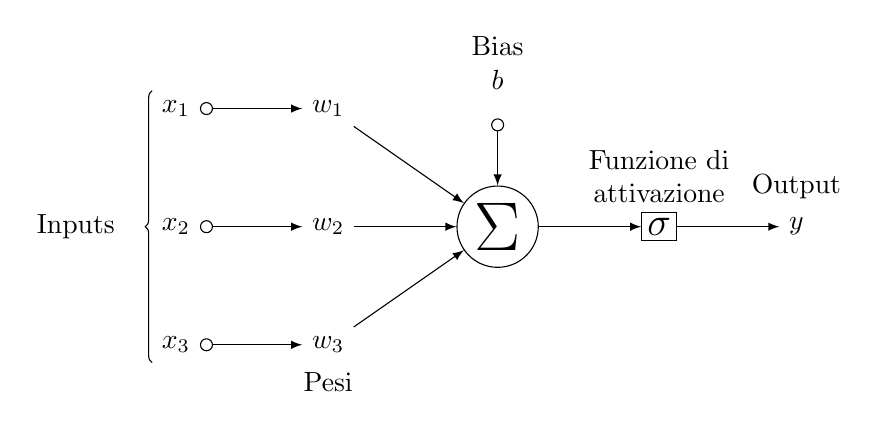
\begin{tikzpicture}[
init/.style={
  draw,
  circle,
  inner sep=2pt,
  font=\Huge,
  join = by -latex
},
squa/.style={
  draw,
  inner sep=2pt,
  font=\Large,
  join = by -latex
},
start chain=2,node distance=13mm
]
\node[on chain=2] 
  (x2) {$x_2$};
\node[on chain=2,join=by o-latex] 
  {$w_2$};
\node[on chain=2,init] (sigma) 
  {$\displaystyle\Sigma$};
\node[on chain=2,squa,label=above:{\parbox{2cm}{\centering Funzione di \\ attivazione}}]   
  {$\sigma$};
\node[on chain=2,label=above:Output,join=by -latex] 
  {$y$};
\begin{scope}[start chain=1]
\node[on chain=1] at (0,1.5cm) 
  (x1) {$x_1$};
\node[on chain=1,join=by o-latex] 
  (w1) {$w_1$};
\end{scope}
\begin{scope}[start chain=3]
\node[on chain=3] at (0,-1.5cm) 
  (x3) {$x_3$};
\node[on chain=3,label=below:Pesi,join=by o-latex] 
  (w3) {$w_3$};
\end{scope}
\node[label=above:\parbox{2cm}{\centering Bias \\ $b$}] at (sigma|-w1) (b) {};

\draw[-latex] (w1) -- (sigma);
\draw[-latex] (w3) -- (sigma);
\draw[o-latex] (b) -- (sigma);

\draw[decorate,decoration={brace,mirror}] (x1.north west) -- node[left=10pt] {Inputs} (x3.south west);
\end{tikzpicture}
 \end{center}

Sempre in formule si può rappresentare l'attivazione del neurone in forma estesa come: 
\begin{equation}
    y = \sigma(w_1  x_1 + w_1  x_1 + .. w_n  x_n + b) = \sigma(\sum_{n=1}^{n} w_n x_n + b)
\end{equation}
La funzione di attivazione è necessaria innanzitutto per trasformare un valore \emph{unbunded}, ovvero senza un valore massimo, derivante dalla sommatoria degli input in un valore continuo che va da 0 a 1, ovvero il valore di attivazione finale che vogliamo fare assumere al neurone del caso. \\
Esistono numerose funzioni di attivazione, una delle più famose e semplici è la \emph{Sigmoide} \[ S(x) = \frac{1}{1+e^{-x}}\] simile alla funzione \emph{gradino unitario} ma in versione smussata, senza la discontinuità nello zero. Questa funzione rispetto al \emph{gradino unitario} ha vari vantaggi, in particolare a piccole variazioni dell'input avremo piccole variazioni nell'output. \\
Nelle reti più moderne è sempre più utilizzata la RELU, ovvero la funzione rettificatore espressa semplicemente come: 
\begin{equation}
     f(x)=\max(0,x)
\end{equation}
Quest'ultima si è dimostrata come la più efficace nelle reti di apprendimento profondo. Fra i suoi vantaggi abbiamo l'attivaazione scarsa, infatti essa si attiva solo nella metà dei campioni di una rete inizializzata casualmente inoltre si hanno meno problemi in fase di discesa del gradiente nella fase di adestramento rispetto alla funzione Sigmoide dei quali parleremo più avanti nel capitolo.
\begin{figure}[h]
\begin{minipage}[t]{0.49\linewidth}
\centering
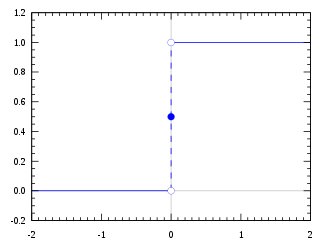
\includegraphics[width=\linewidth]{gradino.png}

(a) Gradino unitario
\end{minipage}%
\hfill\vrule\hfill
\begin{minipage}[t]{0.49\linewidth}
\centering
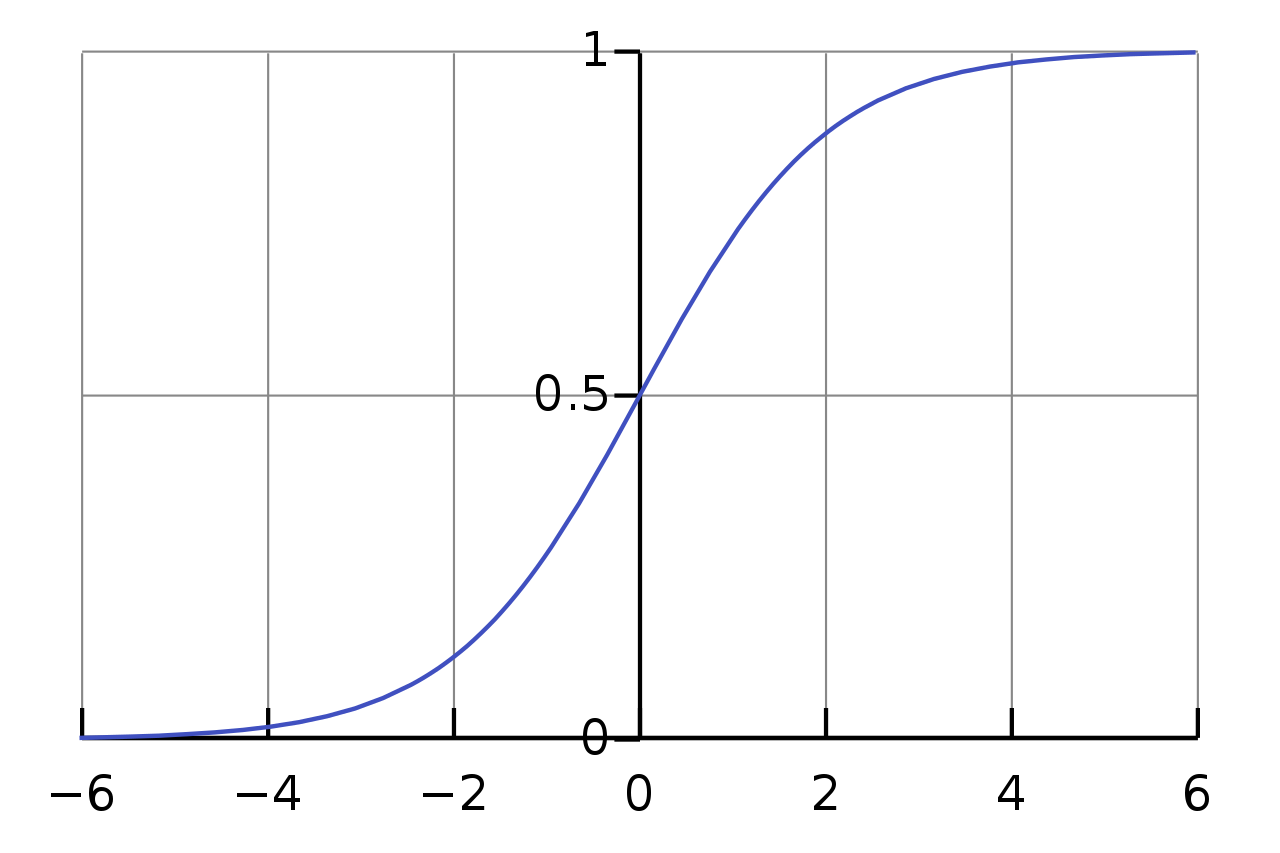
\includegraphics[width=\linewidth]{sigmoid.png}

(b)  Sigmoide
\end{minipage}
\caption{Comparazione fra funzione gradino unitario e sigmoide }
\end{figure}


Esistono poi funzioni di attivazione più sofisticate, come la Softmax.
Quest'ultima è spesso utile nelle reti classificatrici multiclasse. In questi casi i nodi del layer di output rappesentano le probabilità di classificazione per ciascuna classe. In questi casi è cruciale che la sommatoria dei valori di attivazione dei nodi di output sia uguale a 1.
\newpage
Nel caso generale abbiamo almeno un layer di nodi di input, uno di output e acluni layer intermedi detti \emph{hidden-layer}.
In una rete \emph{fully-connected} tutti i nodi nell n-esimo layer sono connessi a tutti i nodi dell'n-esimo layer. \\
Le feature dei vari pattern estrapolati dalla rete vengono calcolati dai nodi dei layer interni i quali estrapolano propietà sempre più astratte e di alto livello quanto più è avanzata la posizione del layer in cui risiedono. \\
Il vettore dei valori di attivazione di un \emph{hidden-layer} può essere espresso come il prodotto tra la matrice dei pesi del layer in questione e il vettore di attivazione del layer precedente più il vettore dei bias, tutto dentro la funzione di attivazione scelta per questo layer.

\begin{figure}[h]
\centering
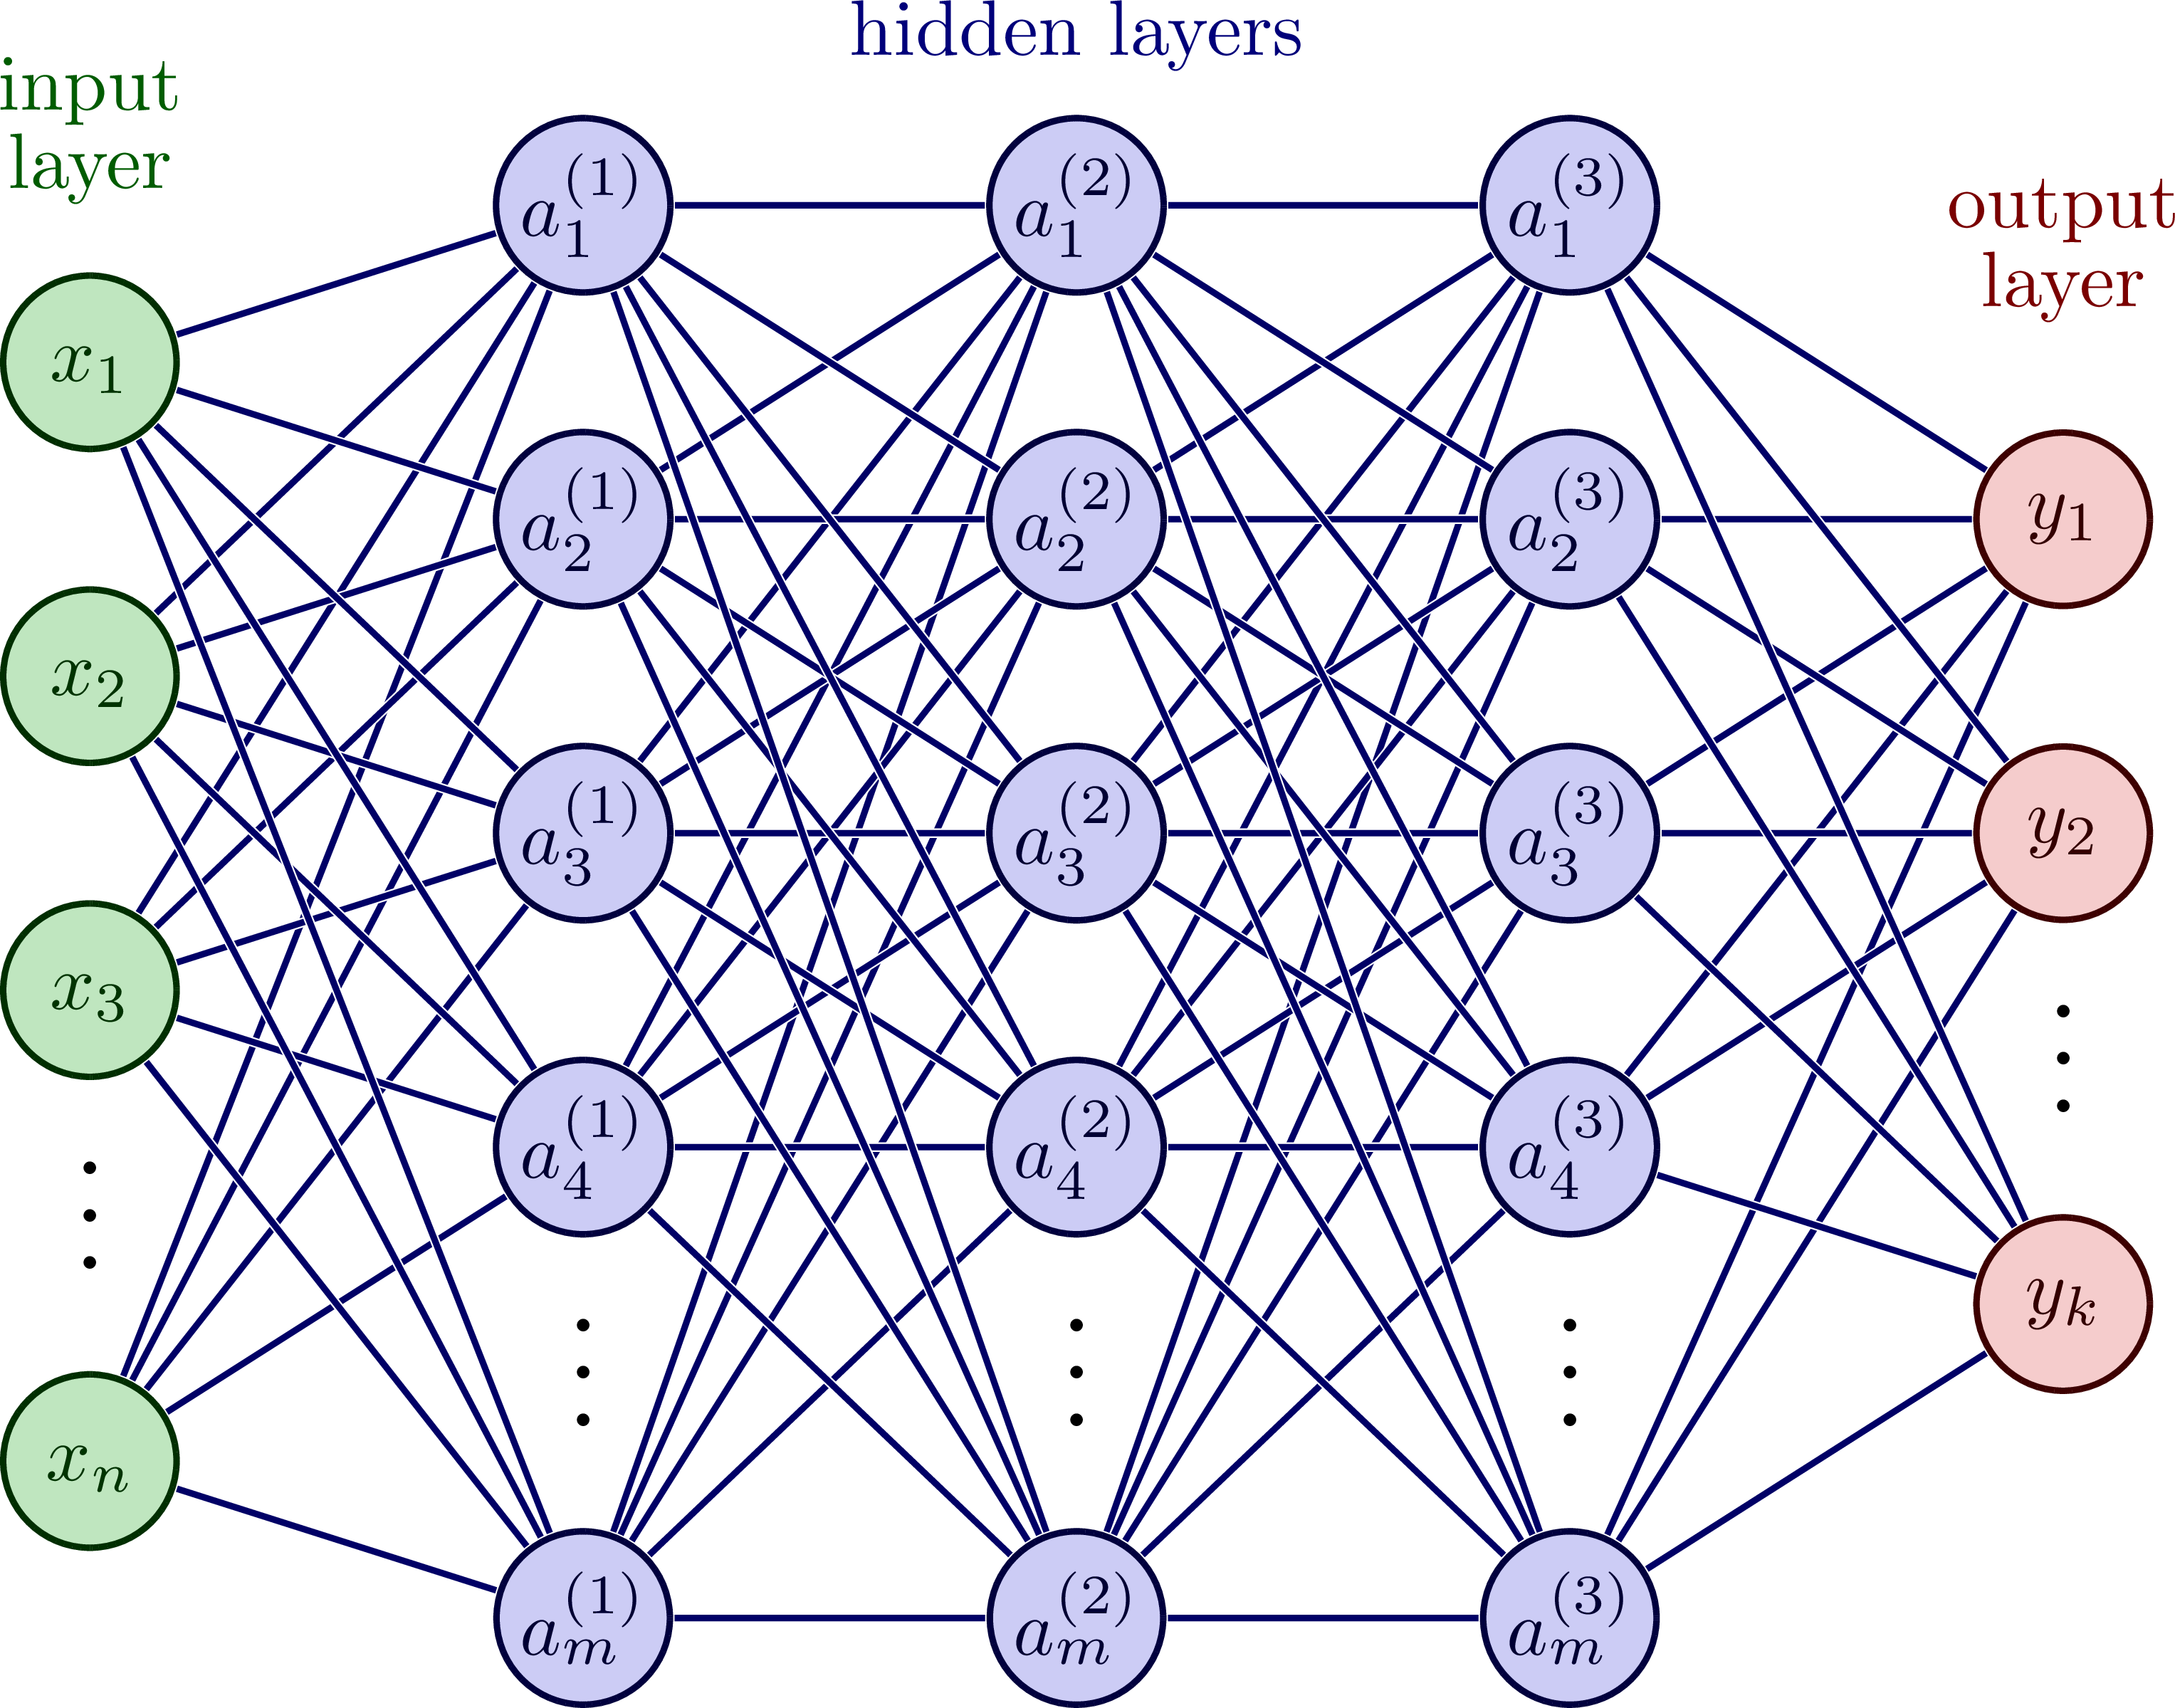
\includegraphics[width=\linewidth]{neural_networks-004.png}
\caption{Rete neurale \emph{fully-connected} con $3$ \emph{hidden layers} da $m$ nodi ciascuno.}
\end{figure}

\newpage
In formule il vettore dei valori di attivazione del primo \emph{hidden-layer} può essere espresso come:
    \begin{equation} 
     \begin{pmatrix}
        a_{1}^{(1)} \\[0.3em]
        a_{2}^{(1)} \\
        \vdots \\
        a_{m}^{(1)}
      \end{pmatrix}
    =
      \sigma \left[ 
      \begin{pmatrix}
        w_{1,0} & w_{1,1} & \ldots & w_{1,n} \\
        w_{2,0} & w_{2,1} & \ldots & w_{2,n} \\
        \vdots  & \vdots  & \ddots & \vdots  \\
        w_{m,0} & w_{m,1} & \ldots & w_{m,n}
      \end{pmatrix}
      {
      \begin{pmatrix}
        a_{1}^{(0)} \\[0.3em]
        a_{2}^{(0)} \\
        \vdots \\
        a_{n}^{(0)}
      \end{pmatrix}}
      +
      \begin{pmatrix}
        b_{1}^{(0)} \\[0.3em]
        b_{2}^{(0)} \\
        \vdots \\
        b_{m}^{(0)}
      \end{pmatrix}\right] 
      \\
    \end{equation}
In notazione compatta abbiamo: 
    \begin{equation}
        \mathbf{a}^{(1)} = \mathbf{W}^{(0)} {a^{(0)}}+\mathbf{b}^{(0)}
    \end{equation}

In generale non tutti le reti sono \emph{fully-connected}, spesso si opta per una soluzione ibrida dove si utilizzano strati con architetture diverse per risolvere un problema. 
Un esempio di un'altra archiettura di rete sono le reti ricorsive (RNN), queste hanno dei collegamenti in retroazione capaci di mantenere uno \emph{stato} e quindi avere \emph{memoria}. Mantenere una memoria è cruciale quando gli imput passati in precedenza nella rete in relazione con quelli attuali hanno un significato semantico importante, come per esempio nell'analisi di un video o per un riconoscimento vocale partendo da un file audio.
Un'altro tipo di rete molto importante e centrale in questo lavoro di tesi sono le reti convoluzionali CNN. Esse si basano su filtri convoluzionali che collegano gli \emph{hidden-layer}.\\ Queste reti riescono a estrapolare pattern grafici a partire da un'immagine fornita come imput, per esempio utilizzando il valore numerico associato ad ogni pixel in un'immagine in scala di grigi.\\
Questo tipo di reti sono state usate nell'ambito di questo progetto per identificare automaticamente le aree di interesse dove sono presenti i difetti del grafene. Di queste reti e in particolare di YOLOv8 ne parleremo nel dettaglio nel prossimo capitolo.

\newpage
\section{Algoritmi di apprendimento}
\subsection{Funzione di costo}
Uno dei parametri più importanti nonchè alla base degli algoritmi di apprendimento è la cosidetta \emph{funzione di costo}.
Ne esistono di vari tipi ma intuitivamente essa è una funzione reale che prende come variabili i parametri del sistema $C(\omega,b)$ e fornisce un'indicazione su quanto bene la nostra rete stia performando sui campioni che gli vengono dati.\\
Questa valutazione è possibile confrontando i valori $y(x)$ che la rete produce per gli imput $x$, conoscendo il vettore $a(x)$ dei risultati attesi per gli imput in questione.
Una delle più utilizzate è lo \emph{scarto quadratico medio}, essa fa la media aritmetica del quadrato dell'errore di output rispetto a ogni imput.
\begin{equation}
    C(\omega,b) = \frac{1}{n} \sum_{n=1}^{n} (y(x_{i}) - a_{i}))^2
\end{equation}
Al variare dei numerosi parametri $(W,b)$ la performance della rete varia e così anche la funzione di costo. In particolare più il valore si avvicina a zero e più la rete sta performando bene. \\
Risulata quindi chiaro che minimizzare la funzione di costo $C(\omega,b)$ è il fulcro del problema dell'addestramento delle reti neurali.
\subsection{Discesa del gradiente}
Siamo quindi di fronte a un problema di ottimizzazione di una funzione reale in tante variabili quanti sono i parametri della rete, dove si cerca quindi un minimo della funzione stessa.
Intuitivamente l'inverso del gradiente ci da un'indicazione \emph{spaziale} su dove dobbiamo \emph{muoverci} per avvicinarci il più velocemente possibile al più vicino minimo locale, quindi per quale vettore di valori dobbiamo sommare i nostri parametri $(\omega,b)$ per migliorarli. \\
\newpage
Le iterazioni del metodo si presentano nella forma seguente: prima si va a calcolare l'inverso del gradiente, lo si moltiplica per una certa costante $\eta$, quindi lo si somma ai parametri $(\omega,b)$. In questo modo si vanno ad ottenere i nuovi parametri $(\omega', b')$. \\
L'equzione seguente mostra un'iterazione del processo di discesa del gradiente, dove vengono calcolati i nuovi parametri $(\omega', b')$:
\begin{equation}
    (\omega', b') := (w,b)-\eta \nabla C(w,b)
\end{equation}
Importante notare come l'entità dello \emph{spostamento} per ogni step è arbitrariamente piccola rispetto al valore di $\eta$. Quest'ultimo prende il nome di \emph{learning-rate} ed è un \emph{iperparametro} in quanto è una variabile scelta a priori da colui che sta addestrando la rete. \\
Un'altro accorgimento per evitare fluttuazioni imprevedibili dei parametri è quello di non applicare i cambiamenti ad ogni predizione ma fare la media su un batch di più predizioni. \\
Il metodo illustrato sopra prende il nome di \emph{Gradient Descent GD}\cite{K1}, questo è un metodo applicabile quando la funzione di costo è sufficientemente semplice e il suo gradiente è di facile computazione.\\
Nel \emph{GD} si calcola il gradiente per l'intero set di parametri ed essi vengono aggiornati ad ogni iterazione oppure facendo la media su batch di un certo numero di predizioni. \\
Quando invece ho dataset molto grandi oppure non ho un'espressione della funzione di costo abbastanza semplice si può optare per il metodo noto come \emph{Stochastic Gradient Descent SGD}.
Questo metodo approssima il calcolo del gradiente considerando ogni volta un batch casuale di paramertri ad ogni iterazione, solo una parte dei parametri quindi vengono aggiornati durante un'iterazione.
\begin{figure}[h]
\centering
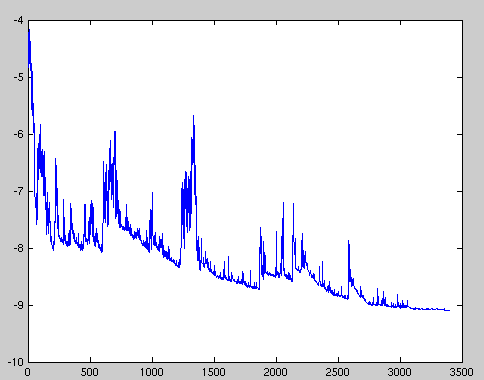
\includegraphics[width=\linewidth]{Stogra.png}
\caption{Esempio di andamento della funzione costo nel corso delle iterazioni in un problema di ottimizzazione risolto tramite SGD}
\end{figure}
\newpage
Come si può vedere dall'andamento della funzione di costo durante le iterazioni del SGD, non è assicurato il miglioramento della rete ad ogni iterazione, in alcuni casi infatti la funzione di costo può momentaneamente salire, questo è dovuto alla natura stocastica, quindi probabilistica del metodo.\\
In generale comunque, per computare la derivata parziale di un parametro occorre un passaggio e il tutto deve essere ripetuto per ogni epoca. \\
Avendo spesso miliardi di parametri e centinaia di epoche i metodi di GD possono risultare facilemente costosi computazionalemente. \\
Per mitigare questo è stato creato un nuovo algoritmo utilizzabile insieme al SGD, esso prende il nome di \emph{Backpropagation}\cite{backprop}.
Questo algoritmo ricorsivo sfruttando la regola della \emph{chain rule} (durante il calcolo del gradiente) permette di calcolare tutte le derivate e quindi l'intero gradiente in un singolo passaggio.\\

Qui sotto mostro la differenza intuitiva fra la progressione di un algoritmo di GD a batch con uno di SGD.\\
Notare bene come la visualizzazione è possibile solo se si considera il caso estremamente semplificato di soli due parametri. \\Nel caso generico con più di due parametri (anche miliardi) sarebbe impossibile proporre una visualizzazione di uno spazio con così tante dimensioni.
\begin{figure}[h]
\begin{minipage}[t]{0.49\linewidth}
\centering
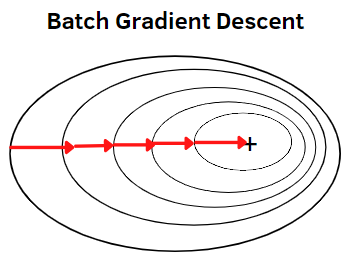
\includegraphics[width=\linewidth]{batchGD.png}

(a) Batch Gradient Descent
\end{minipage}%
\hfill\vrule\hfill
\begin{minipage}[t]{0.49\linewidth}
\centering
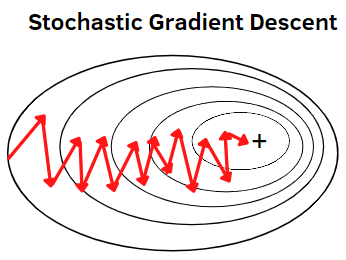
\includegraphics[width=\linewidth]{SGD.png}

(b)  Stochastic Gradient Descent
\end{minipage}
\caption{Comparazione fra iterazioni di GD a batch e SGD }
\end{figure}
Notare la natura intrisecamente probabilistica degli step del SGD, essi non assicurano un miglioramento della loss ad ogni step ma il risulato finale può risultare comunque più efficente della controparte GD se analizzato nel complesso.
\newpage

\section{Esempi applicativi di Reti Neurali}
Le reti neurali hanno numerose ricadute per la risoluzione di problemi applicativi di ogni genere.
Forse il più famoso caso applicativo in letteratura e sicuramente il più usato per introdurre le Reti Neurali Convoluzionali (\emph{CNN}) è il problema del riconoscimento automatico di numeri (cifre) scritte a mano. 
Le CNN verranno approfondite nel prossimo capitolo, in particolare verranno inquadrate nella classe di problemi di Object Detection, ma vale comunque la pena introdurre fin da subito la risoluzione di questo ben noto caso di studio. 
\subsection{Classificazione di cifre scritte a mano}

Il dataset di riferimento è il ben noto \emph{MNIST}.\\
Le immagini contenute rappresentano semplici numeri a una cifra scritti a mano, ognuno di questi viene fornito con la relativa annotazone (\emph{label}) scritta da operatori umani.\\
Questo database contiene 60.000 immagini 28x28 pixel in scala di grigi per la fase di training e ulteriori 10.000 per la fase di valutazione del modello. \\
\begin{figure}[h]
\centering
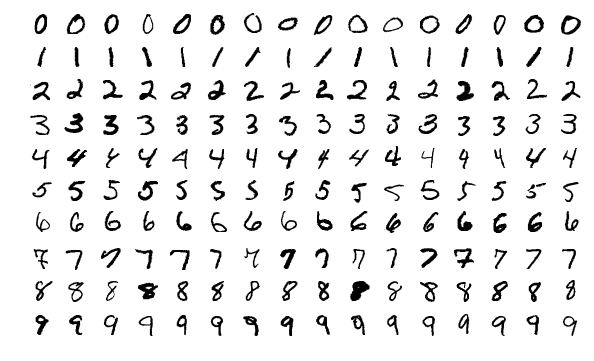
\includegraphics[width=\linewidth]{minst.png}
\caption{Database MINST}
\end{figure}
La valutazione di ogni modello di reti neurali non deve essere effettuata sugli stessi dati di addestramento, ma su altri che il modello non ha mai visto prima. Ciò che si vuole valutare infatti è la capacità acquisita dal sistema nel riconoscimento di pattern generali estrapolabili da campioni generici. Se utilizzassimo gli stessi dati usati nell'adestramento per valutare la rete, rischieremmo di incorrere nella possibilità che la rete sia performate nell'analisi dei dati di training ma incapace di generalizzare su dati generici mai visti prima.   \\
\newpage
L'imput layer è composto da tanti nodi quanti sono i pixel dell'immagine, ognuno di questi prende il valore numerico in scala di grigi del pixel in questione.
L'imput layer quindi, si deve pensare come la matrice di pixel dell'immagine iniziale. Nel caso avessimo un'immagine a colori, per esempio in formato RGB, al posto di un imput layer sotto forme di matrice, ne avremo 3, una per ogni colore (rosso, verde, blu), lavoreremo quindi con tensori.\\
\newpage
\begin{figure}[h]
\centering
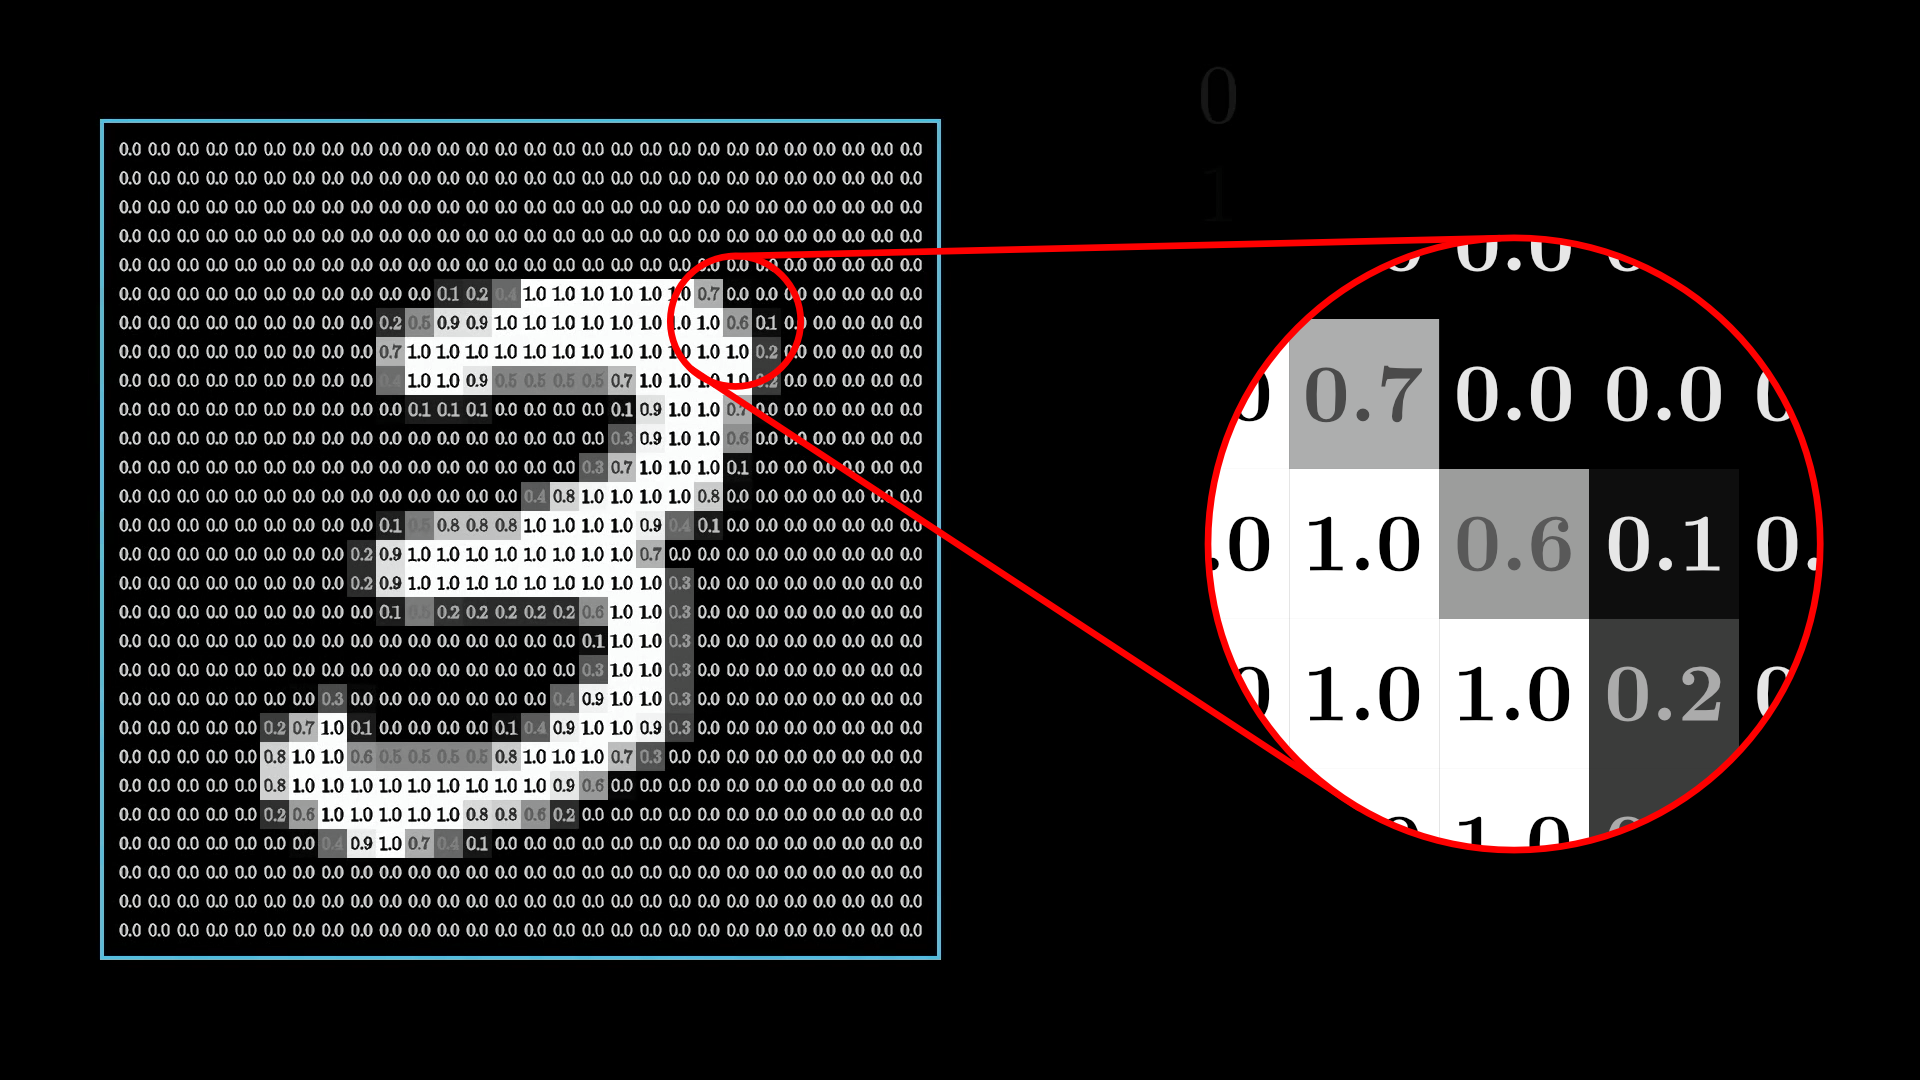
\includegraphics[width=\linewidth]{pixel-values.png}
\caption{Imput layer di una CNN per analisi immagine}
\end{figure}
Questo problema, come in tutti i casi in cui si cercano oggetti e/o pattern all'interno di immagini, si risolve impiegando strati convoluzionali. \\
Questi strati di neuroni sono composti da \emph{filtri} che \emph{scorrendo} sui valori di attivazione dei layer prededenti computano operazioni di convoluzione estrapolando tratti \emph{grafici} dalle immagini.\\
La natura di questi \emph{filtri} e delle operazioni di convoluzione effettuate da essi verranno approfonditi e esplorati nel prossimo capitolo. 
In generale ci aspettiamo che layer convoluzionali di strati più avanzati estrapolino tratti grafici più astratti e complessi sulla base dei tratti di più basso livello estratti dai livelli inferiori. Nel nostro caso è plausibile che i primi livelli riconoscano feature di basso livello come i bordi delle cifre, mentre quelli successivi riconoscano pattern più strutturati come per esempio i \emph{cerchi} dello zero e dell'otto. 
\newpage

\begin{figure}[h]
\centering
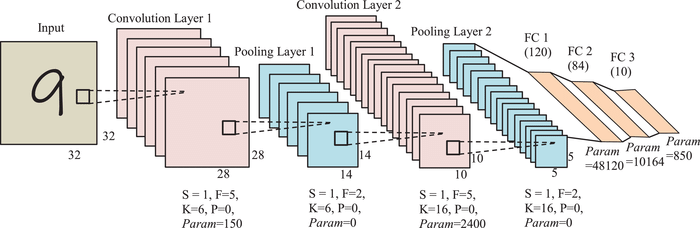
\includegraphics[width=\linewidth]{digit_arch.png}
\caption{Modello di CNN per riconoscimento di cifre scritte a mano}
\end{figure}
Come mostrato in figura, spesso fra un layer convoluzionale e il successivo sono presenti dei layer di altra natura, come quelli di \emph{pooling}. Ne esistono di vari tipi ma anchessi si comportano come dei filtri che scorrono sulle immagini prodotte dai filtri convoluzionali precedenti. Il loro scopo è quello di diminuire le dimensione delle immagini prodotte mantenedo parte dell'informazone grafica, magari enfatizzando delle strutture geometriche piuttosto che altre.

Gli ultimi layer invece tornano ad essere \emph{fully-connected} e vengono chiamati \emph{DL, Dense Layers.}
In particolare l'ultimo layer si occupa della classificazione della cifra data come input. Come spiegato in precedenza in questi casi si utilizzano funzioni di attivazione con un comportamento similare alla Softmax. La sommatoria dell'attivaizone dei 10 nodi dell'output layer deve essere infatti pari a 1, dato che ciascunio dei valori di attivazione rappresenta la probabilità che l'immagine di imput corrisponda alla cifra simboleggaita dal suddetto nodo.\\
\newpage
In conclusione possiamo dire che l'applicazione di una CNN a questo tipo di problema si rivela la scelta migliore, in generale risulta la scelta più performante in tutti i tipi di probelmi dove l'imput è composto da un'immagine.\\
\begin{figure}[h]
\centering
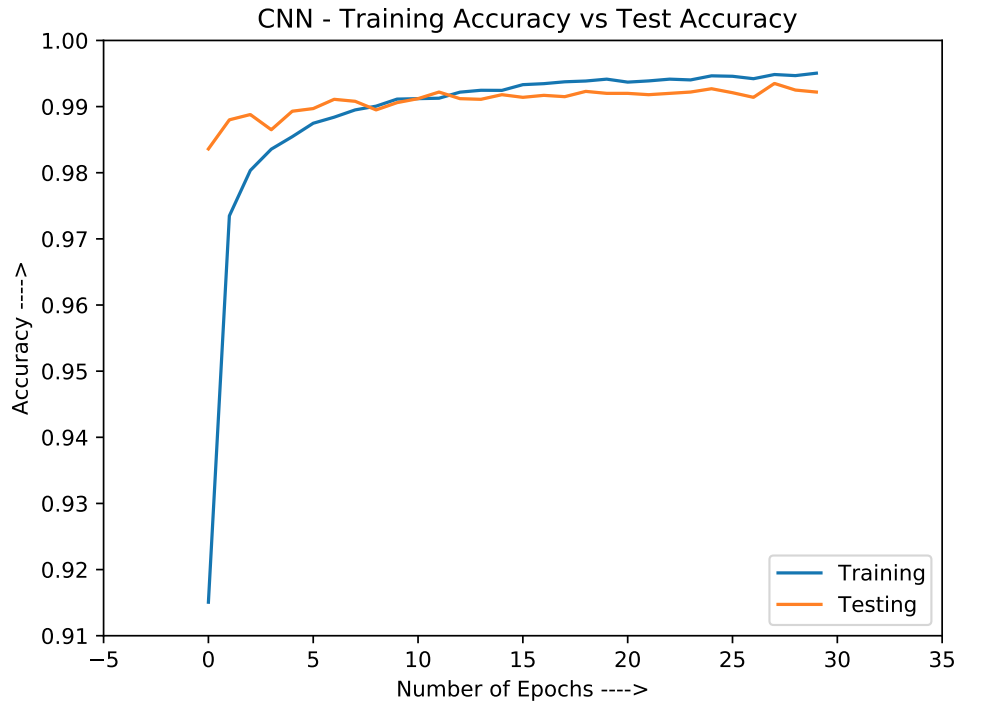
\includegraphics[width=\linewidth]{cnn_perf.png}
\caption{Modello di CNN per riconoscimento di cifre scritte a mano}
\end{figure}
In questo caso di studio già dopo una poche decine di epoche la precisione della classificazione si avvicina al 100\%.
Proseguire oltre non è necessario e anzi può risultare controproducente in quanto si potrebbe andare incontro a problemi di overfitting.
Con overfitting si intende ls situazione in cui il modello si adatta troppo ai dati di training perdendo generalità e capacità di astrarre su dataset mai visti prima. \\

%------------------------------------------------------------------------------------------------------------- CAPITOLO 2 -------------------------------------------------------------------------------------------------
{\let\clearpage\relax \chapter{Object Detection, YOLO e applicazioni su campioni di nano grafene}}

In questo capitolo andremo a introdurre la classe di problemi di visione artificiale denominata come Object Detection. Ovvero le soluzioni e i metodi che puntano a individuare, classificare o comunque riconoscere oggetti e/o pattern all'interno di un'immagine o un video. \\
Questa clase di problemi, come accennato nel capitolo precedete si è rivelata molto adatta all'impiego delle CNN (Convolutional Neural Networks), che grazie alla loro capacità di riconiscemnto ed estrapolazione di fetaures grafiche dalle immagini riescono a ottenere ottime performance su questa classe di problemi.\\
Dopo un'introduzione all'architttura delle CNN, ci focalizzeremo sullo studio di \emph{YOLO (You Only Look Once)}, una CNN allo stato dell'arte per quanto riguarda l'Object Detection, particolarmente nota per il basso tempo di inferenza e per questo particolarmente utile nelle applicazioni in tempo reale.\\
Analizzeremo inoltre l'applicazione di questo modello al caso di studio del progetto su cui si basa questa tesi, ovvero sul riconoscimento automatico di difetti su campioni di nano grafene, riportando metodologia e risultati.
\section{Reti neurali convoluzionali}
La struttura delle CNN è composta da vari tipi di layer di natura diversa, come i layer convoluzionali, i pooling layer e i fully-connected layers. 
Ogni tipologia di layer svolge ruoli e opera in modo diverso rispetto agli altri al fine di raggiungere l'obbiettivo preposto.
\\L'architettura generale può essere espressa come come nella figura sottostante.\\

\begin{figure}[h]
\centering
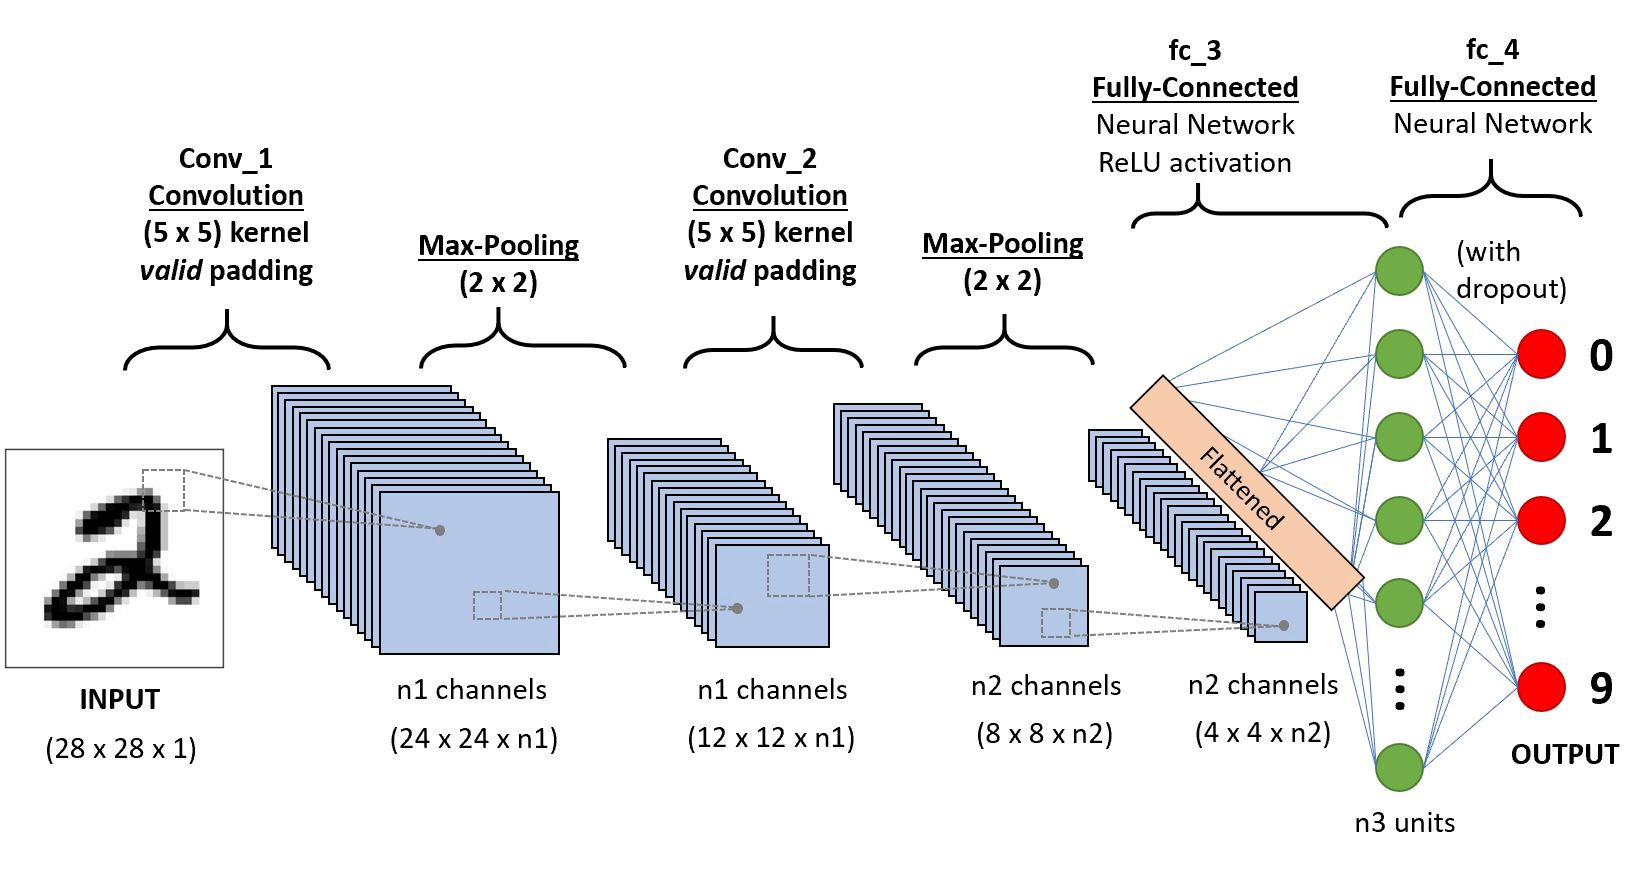
\includegraphics[width=\linewidth]{CNN_main.jpeg}
\caption{Archiettura di una CNN a singolo canale}
\end{figure}
In questa trattazione delle CNN ci limiteramo ad analizzare il caso in cui l'immagine di input sia in scala di grigi e quindi il layer di input sarà composto da matrice di interi con valori compresi tra 0 e 255.
Nonostante questa semplificazione è importante sapere che il tutto può essere esteso ad immagini a più canali introducendo ulteriori matrici, una per ogni canale aggiuntivo. Generalmente quindi si avranno tensori con 3 dimensioni di profondità. 
\newpage
\begin{figure}[h]
\centering
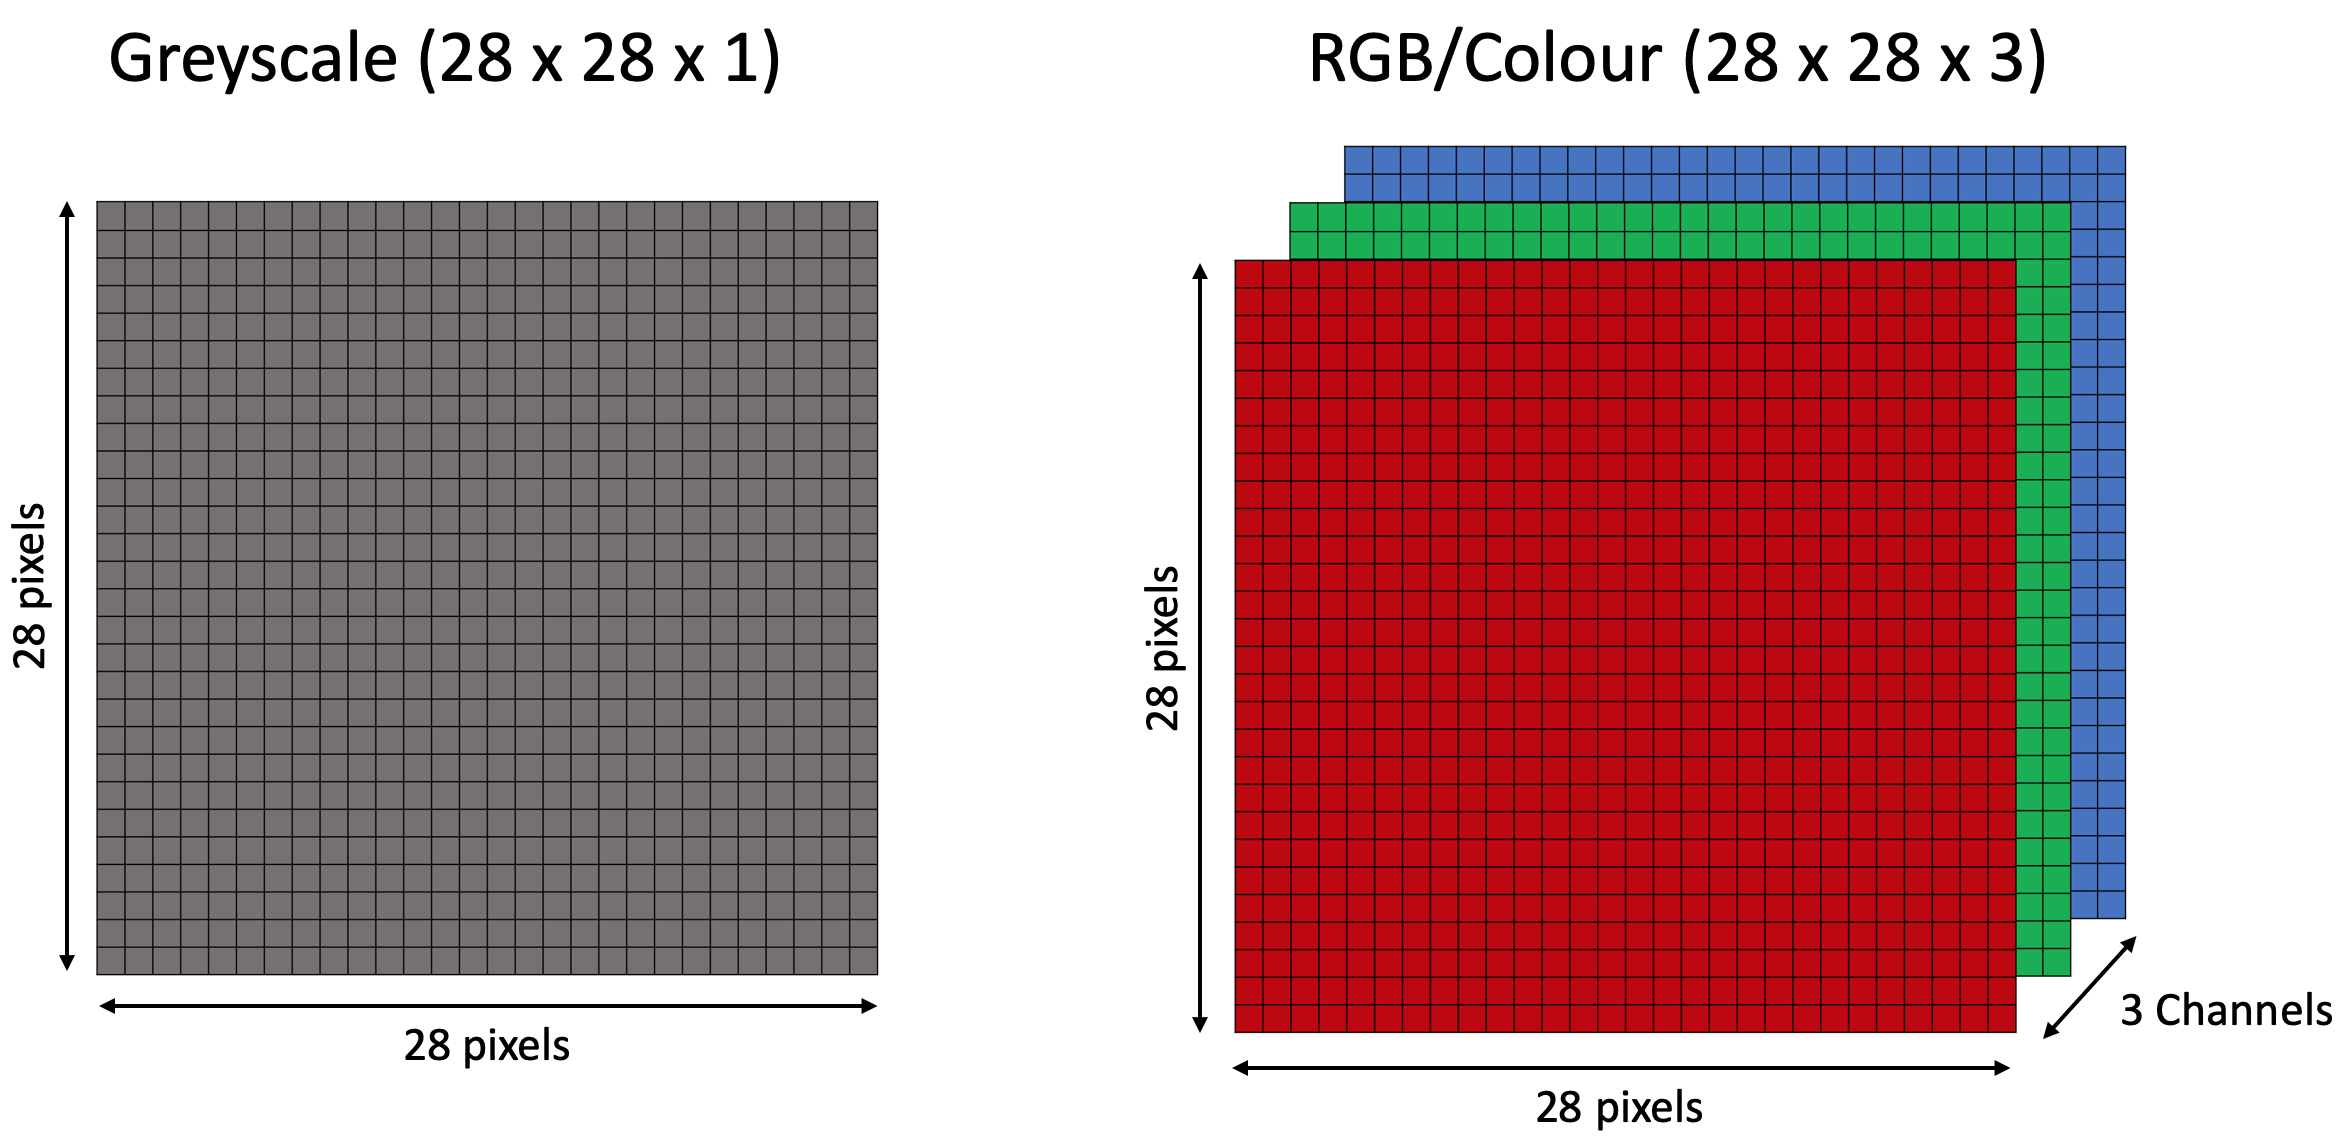
\includegraphics[width=\linewidth]{greyscaletorgb.png}
\caption{Passaggio da matrice di imput in scala di grigi a tensore per immagine RGB}
\end{figure}

In questa sezione andremo ad analizzare un tipo di layer alla volta, iniziando dai layer convoluzionali.
\subsection{Layer convoluzionali}
I componenti fondamentali dei layer convolzuonali non sono più vettori di neuroni ma fetaure map (matrici o tensori) computate da dei \emph{filtri} tramite operazioni di convoluzione discreta.
Questi filtri si presentano come delle matrici di dimensione minore della matrice di input, il loro comportamento è quello di \emph{scorrere} su tutta l'immagine di partenza andando a creare un'altra matrice, di dimensione minore chiamata \emph{feature map.}
L'operazione di convololuzione si può esprimere com la sommatoria del prodotto puntuale di ogni valore del filtro con i rispettivi valori nella matrice di partenza, secondo la posizione del filtro.
\newpage
In formule posiamo indicare l'attivazione di ogni nodo (pixel) della feature map come: 
\begin{equation}
    o_{i,j} = \sigma(b + \sum _{l=0}^{n}\sum _{m=0}^{n}\omega_{l,m}a_{i+l, j+m})
\end{equation}
dove $o_{i,j}$ è l'attivazione dell'elemento della matrice di output, $\sigma$ è una qualsiasi funzione di attivazione, $b$ l'eventuale bias, $\omega_{l,m}$ il valore dell'elemento del filtro nella posizione $l,m$ e $a_{i+l, j+m}$ il valore del pixel dell'immagine di input che verrà moltiplicato per $\omega_{l,m}$ durante lo step.

\begin{figure}[h]
\begin{minipage}[t]{0.49\linewidth}
\centering
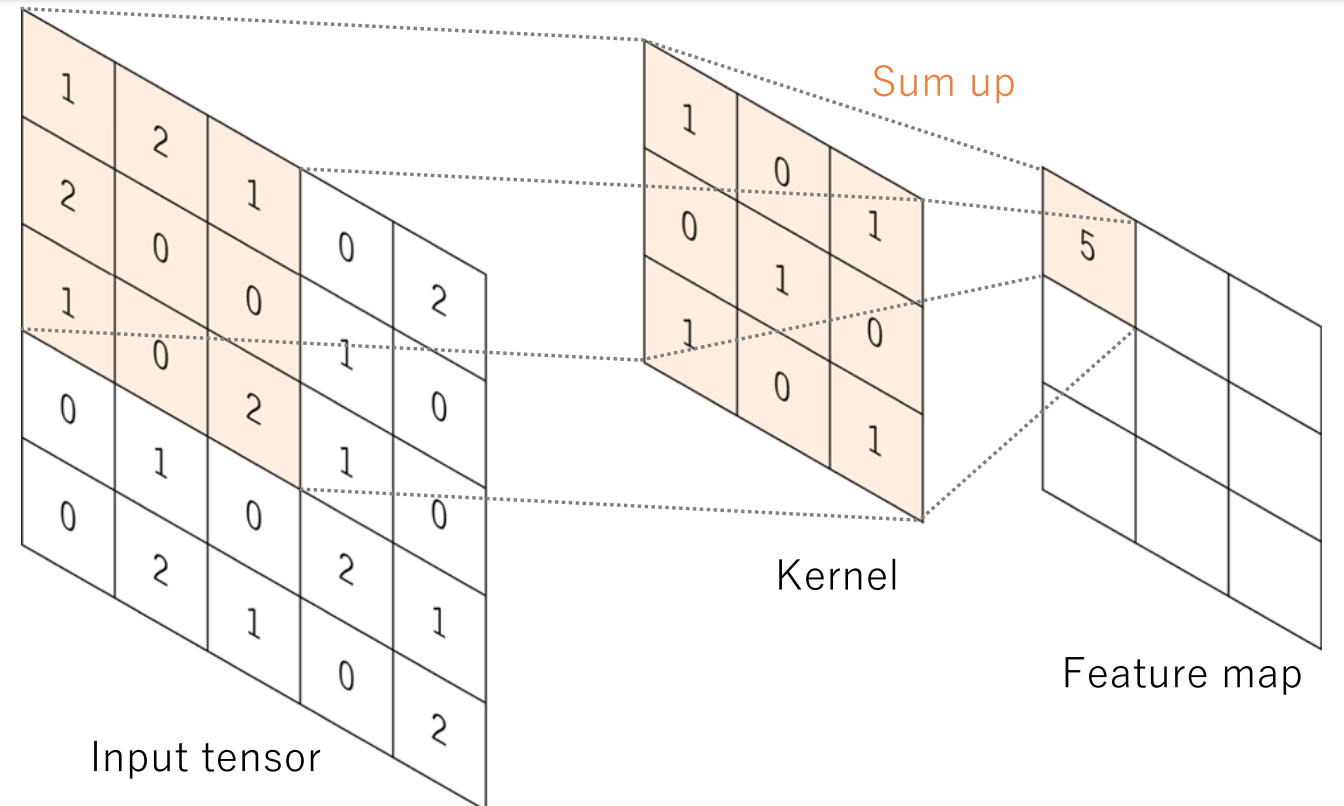
\includegraphics[width=\linewidth]{filtera.png}

(a) Prima convoluzione  
\end{minipage}%
\hfill\vrule\hfill
\begin{minipage}[t]{0.49\linewidth}
\centering
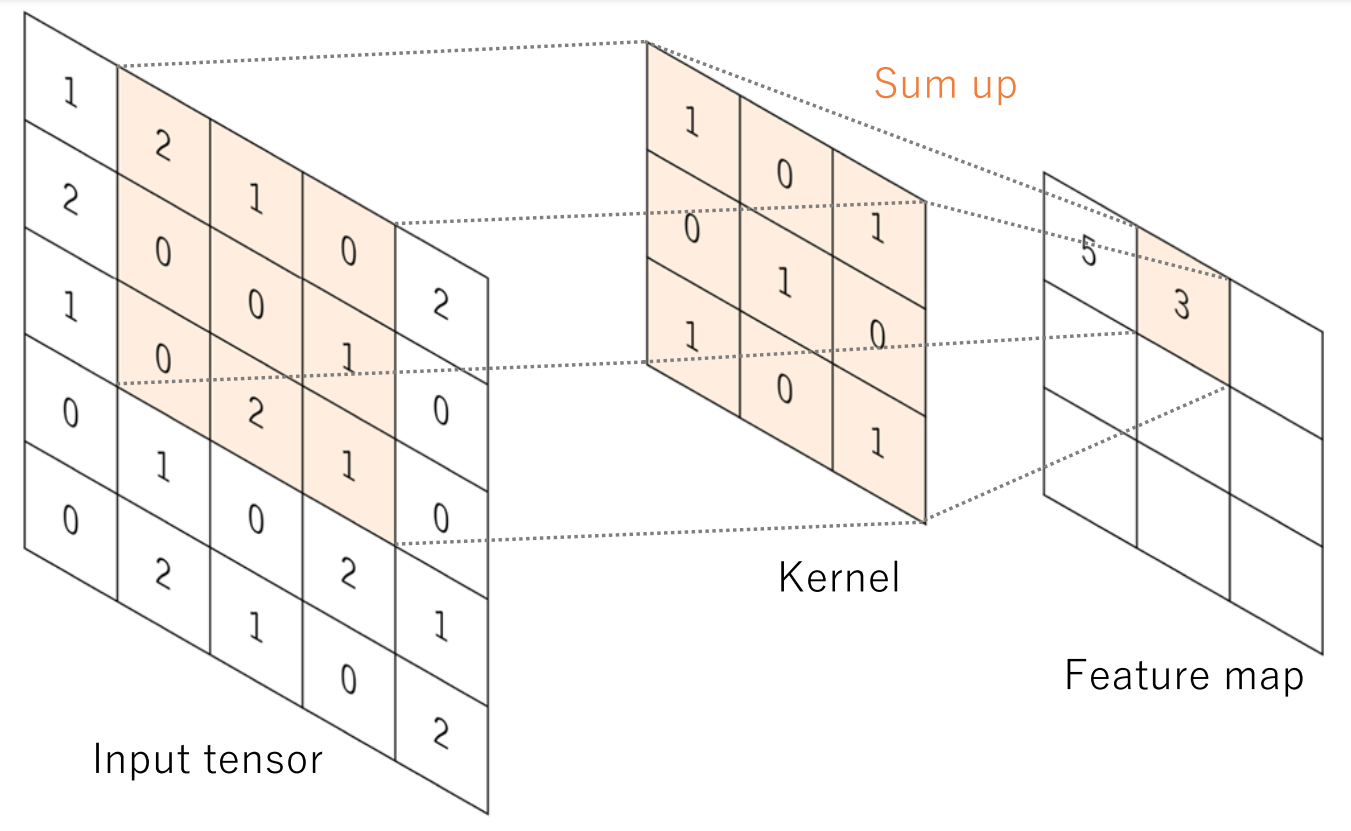
\includegraphics[width=\linewidth]{filterb.png}

(b) Seconda convoluzione
\end{minipage}
\caption{Prime due iterazioni di convoluzione per la creazione di una feature map, con un filtro 3x3, no padding e stride 1}
\end{figure}
La feature map prodotta risulta più piccola dell'immagine di partenza, questo può essere un problema se si applicano numerose convoluzioni in sequenza andano quindi a ridurre sempre di più la dimensione delle immagini prodotte. Per evitare questo si può applicare la tecnica chiamata \emph{padding}, ovvero l'aggiunta a  posteriori di uno strato esterno alla matrice dell'immagine con valori nulli (\emph{zero padding}. Allo scorrere del filtro quindi si otterrà un'immagine della stessa dimensione di partenza.\\
Lo \emph{stride} invece è la dimensione dello \emph{step} del filtro durante lo scorrimento, solitamente è pari a 1, se lo si aumentasse si otterebbero anche in questo caso feature map più piccole dell'originale.

Questi filtri nei primi layer sono in grado di estrarre tratti di basso livello come i bordi e contorni degli oggetti. In generale sono molto adatti per enfatizzazione contorni di oggetti sull'immagine di partenza in modo da rendere più facile le operazioni dei layer successivi.
Nell'immagine successiva si mostrano varie feature map derivate da diversi filtri diversi. E' chiaro come l'operazione di convoluzione applicata da specifici filtri sia in grado di mettere in risalto contorni diversi rispetto ad altri.
\begin{figure}[h]
\centering
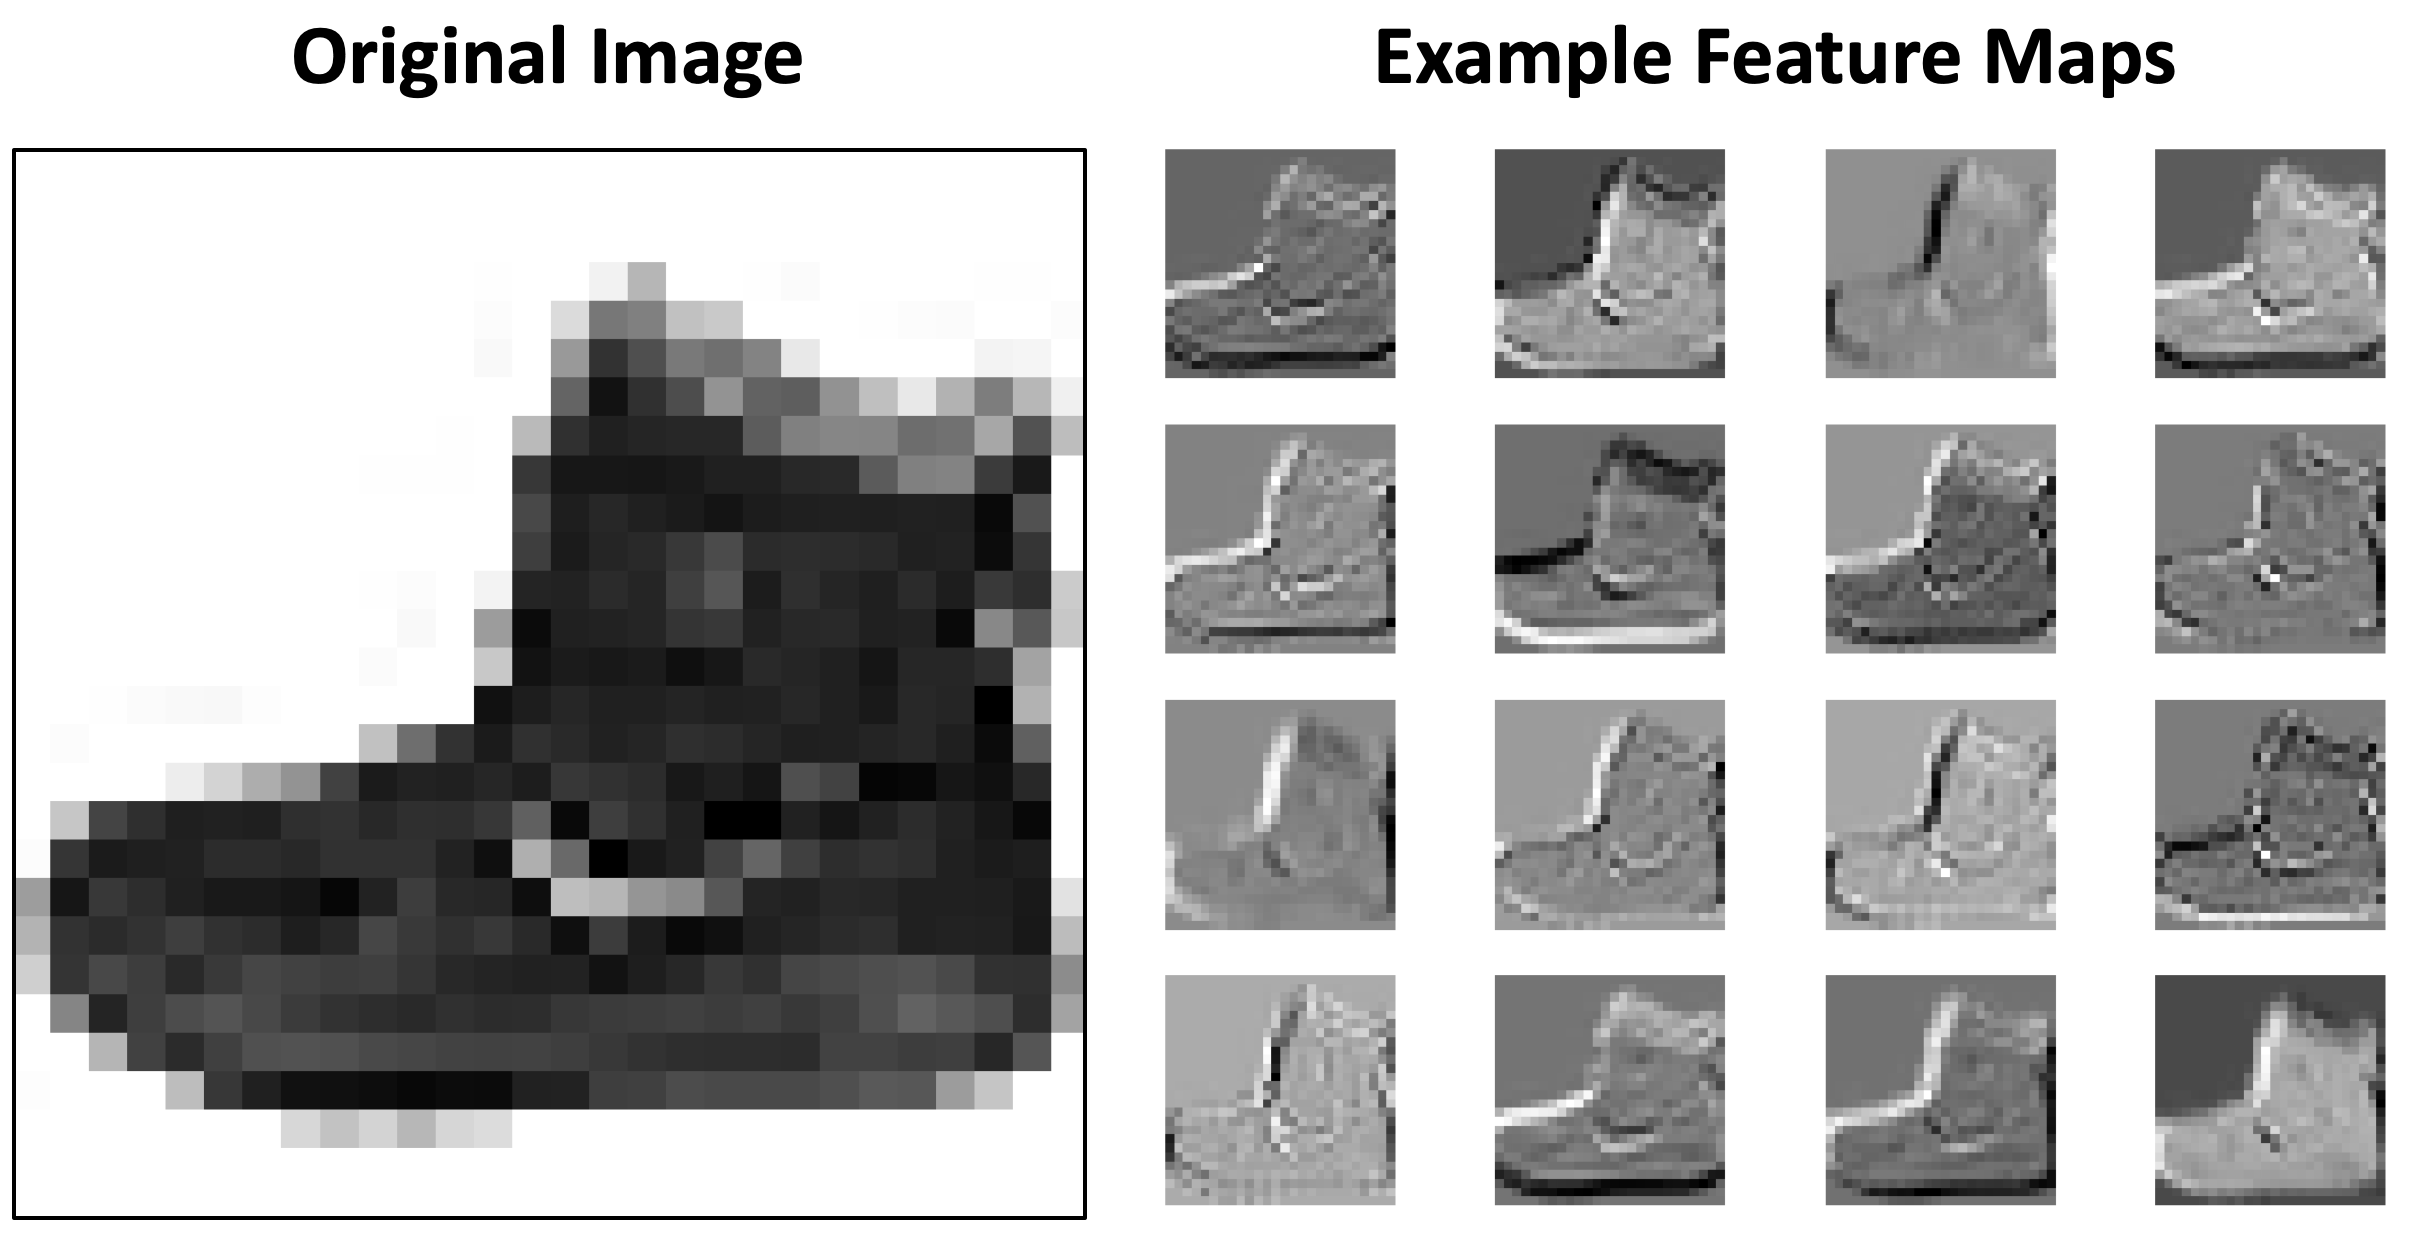
\includegraphics[width=\linewidth]{fetaureMaps.png}
\caption{Fetaure map generate da diversi filtri a sulla stessa immagine}
\end{figure}
Il risulatato dell'operazione lineare di convoluzione viene quindi passato per una funzione di attivazione non lineare come la ReLU, discussa nel capitolo precedente.\\

I parametri fondamentali di apprendimento delle CNN sono propio i pesi (quindi gli elementi di matrice) dei filtri convoluzionali, la rete quindi apprenderà i valori ottimali per ciascun filtro allo scopo di estrapolare i pattern richeisti dal problema.
\\
Invece, la dimensione e il numero dei filtri, il padding e lo stride sono \emph{iperparametri}, ovvero sono valori decisi a priori da colui che sta addestrando la rete, prima del processo di training stesso. 
\newpage
\subsection{Layer di pooling}
Dopo una serie di convoluzioni, tipicamente, si va ad applicare un layer di \emph{pooling}, ovvero un'altra operazione lineare simile alla convoluzione dalla quale si ottengono immagini più piccole ma che comunque mantengono un certo contenuto informativo posizionale della feature map iniziale.
Esistono varie tipologie di pooling con comportamenti diversi tra loro, nell'immagine sottostante si mostra il funzioanamento della tipologia di gran lunga più utilizzata, il \emph{Max-pooling}.

\begin{figure}[h]
\centering
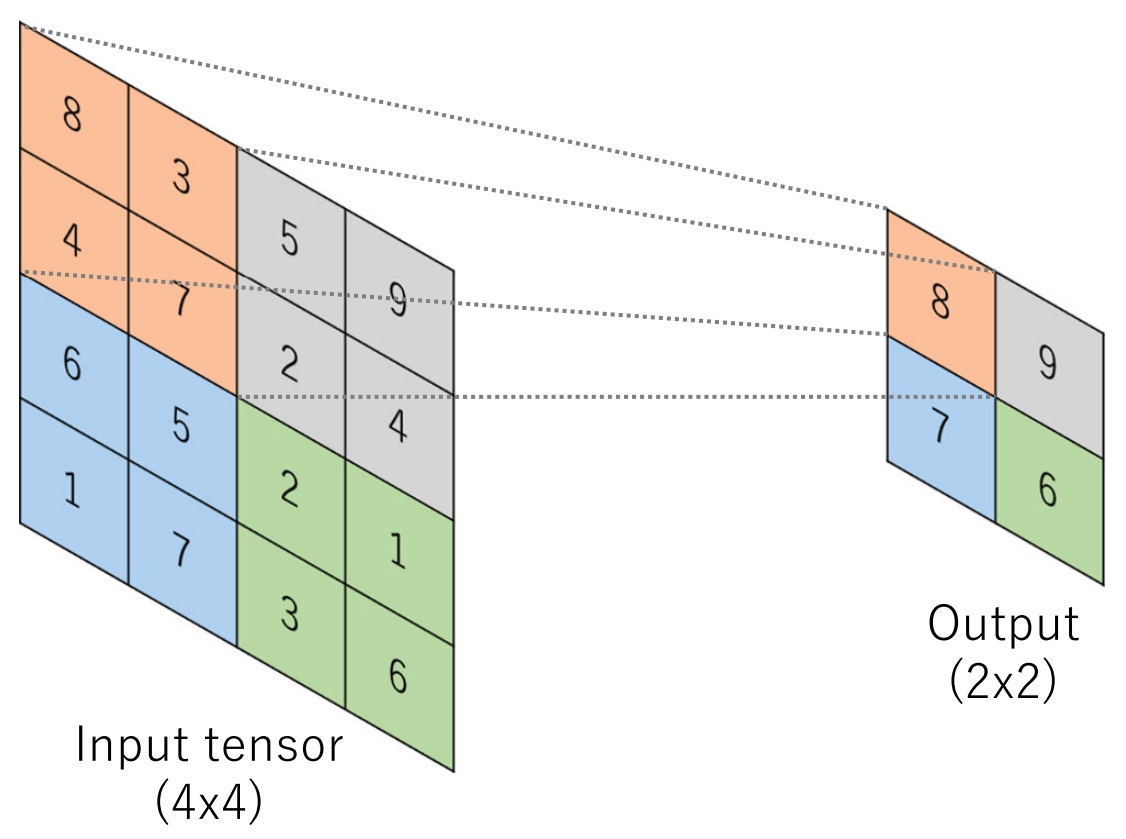
\includegraphics[width=\linewidth]{maxpooling.png}
\caption{Maxpooling 2x2, stride 2}
\end{figure}
Il funzionamento del max-pooling è similare a quello di un filtro convoluzionale che scorre su una feature map, ma al posto di fare la convoluzione dei valori, prende il valore più grande fra quelli coperti dalle dimensioni del filtro e lo riporta nella nuova immagine.\\

Il \emph{pooling}, più in generale, è quindi un processo di scalamento della feature map di partenza introducendo una invarianza a piccole distorsioni e variazioni dell'immagine stessa mantenendo però gran parte delle informazioni spaziali della dell'immagine iniziale.\\
Grazie a questo processo è possibile ridurre notevolemente i parametri di apprendimento della rete. Notare inoltre che i parametri di pooling come dimensione dei filtri, stride e padding sono tutti iperparametri che non vengono appresi dalla rete in fase di training.
\begin{figure}[h]
\centering
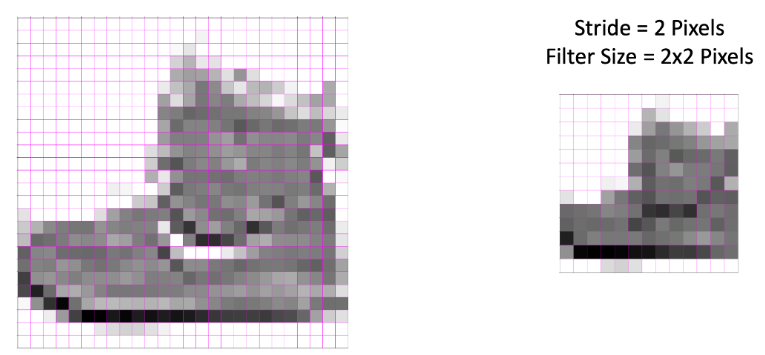
\includegraphics[width=\linewidth]{maxPoolingResult.png}
\caption{Risultato di un'operazione di max-pooling 2x2 con stride 2}
\end{figure}
\\Notare come se si va ad applicare un layer di max-pooling 2x2 con stride 2, la feature map di partenza viene dimezzata come dimensioni ma il contenuto semantico dell'immagine rimane intatto.

\subsection{Fully-connected layer }
Gli ultimi layer della rete sono fully-connected, del tutto simili a quelli introdotti nel capitolo 1. \\
Le feature map prodotte dall'ultimo layer convoluzionale/pooling vengono \emph{appiattite}, ovvero inserite in un semplice array unidimensionale (un vettore) e connessi a uno o più layer fully-connected. In questo layer per ogni connessione fra un neurone e l'altro c'è un peso, che la rete andrà ad apprendere durante l'addestramento, inoltre l'attivazione del singolo neurone viene passata tipicamente attraverso la ReLU. Le feature grafiche estratte dai layer precedenti sono finalmente mappate tramite i layer fully-connected al layer di output che rappresenta le probabilità di classificazione dell'immagine.
\\Il layer di output viene anchesso passato per una funzione di attivazione, tipicamente diversa da quelle utilizzate dei dense-layer precedenti. Nel caso della classificazione multipla si usa la Softmax, nel caso della classificazione binaria la sigmoide.
\begin{figure}[h]
\centering
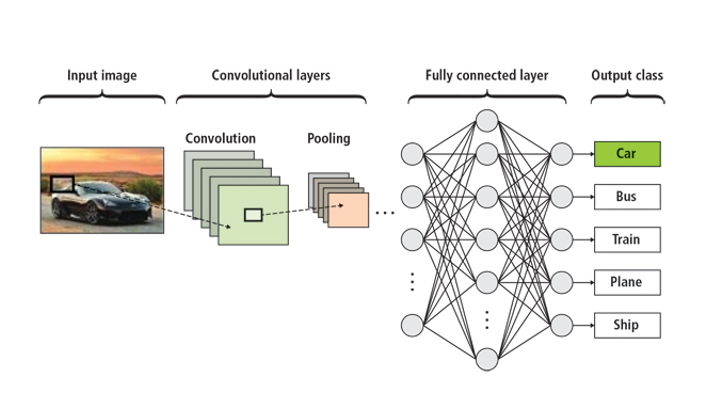
\includegraphics[width=\linewidth]{CNN_fully_connected.png}
\caption{CNN con fully connected layer nella parte finale per classificazione multiclasse di oggetti }
\end{figure}

Nei problemi di classifcazione multiclasse il layer di output può essere trattato come una distribuzione di probabilità. Ovvero la rete non si limita a fornire un giudizio sulla classe presente nell'immagine, ma fornisce una probabilità per ogni classe presente nel problema.
Per valutare la performace della rete è utile quindi confrontare la distribuzione di probabilità prodotta dalla rete con quella attesa.
\newpage
Viene usata quindi una funzione di costo diversa da quella trattata nel primo capitolo, chimata funzione di cross-entropia.
\begin{equation}
    C\left(p\|q\right)=-\sum _{i}^{M}p_{i}\log _{2}q_{i}
\end{equation}
All'interno del contesto di una predizione per un'immagine in input, $M$ rappresenta il numero di classi globali, $p_{i}$ rappresenta il valore della classe $i$ nella distribuzione dei valori attesi, e $q_{i}$ rappresenta il valore della classe $i$ nella distribuzione prodotta dalla rete (predizione).\\
La formuala nel caso pratico dei problemi di clasificazione si semplifica in quanto i valori di $p_{i}$ sono sempre nulli per tutte le classi meno che per la classe effettivamente indicata nella fase di labeling per quell'immagine dove invece è pari a 1. \\ Quindi possiamo riscrivere la formula come: 
\begin{equation}
    C\left(p\|q\right)=-\sum _{i}^{M}\log _{2}q_{i}
\end{equation}
\begin{figure}[h]
\centering
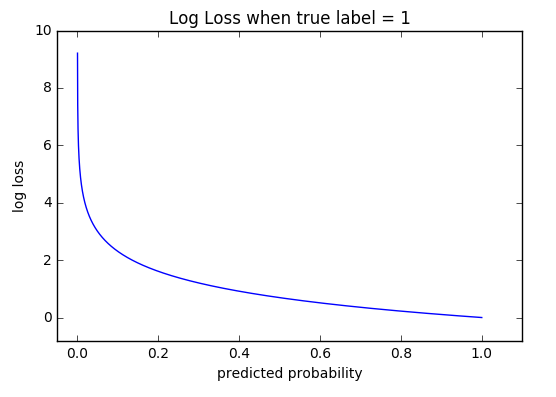
\includegraphics[width=\linewidth]{cross_entropy.png}
\caption{Comportamento della funzione di costo in base alle predizioni del modello}
\end{figure}
La cross-entropy si è rivelata molto adatta nei problemi di classificazione multiclasse per la sua rapida pendenza nei casi in cui la rete assegna una scarsa probabilità alla classe presente nel'immagine. In questi scenari infatti le magnitudine delle sue derivate inducono a rapide variazioni dei parametri di apprendimento. In questo modo gli algoritmi di ottimizzazione riescono a migliorare le performace della rete con rapidità.
\newpage
Concludo la sezione osservando che nelle CNN è fondamentale scegliere a priori un buon set di iperparametri e di architettura dei layer adatto per risolvere il problema in questione, compresa la funzione di costo e l'ottimizzatore. \\

Nella prossima sezione andremo ad analizzare il problema dell'Object Detection e l'architettura di una nota rete di Object Detection, YOLO.
\newpage
\section{Object Detection}
I problemi di Object Detection consistono nel volere individuare da un'immagine data come input uno o più oggetti, disegnando rettangoli che li ricoprono completamente, chiamati \emph{bounding boxes}. Inoltre, nel caso di un problema multiclasse, il modello dovrà classificare correttamente l'oggetto trovato tra le varie classi possibili. Dunque, viene fornito anche un valore numerico compreso tra 0 e 1 che rappresenta la confidenza del modello per la suddetta predizione.
\begin{figure}[h]
\centering
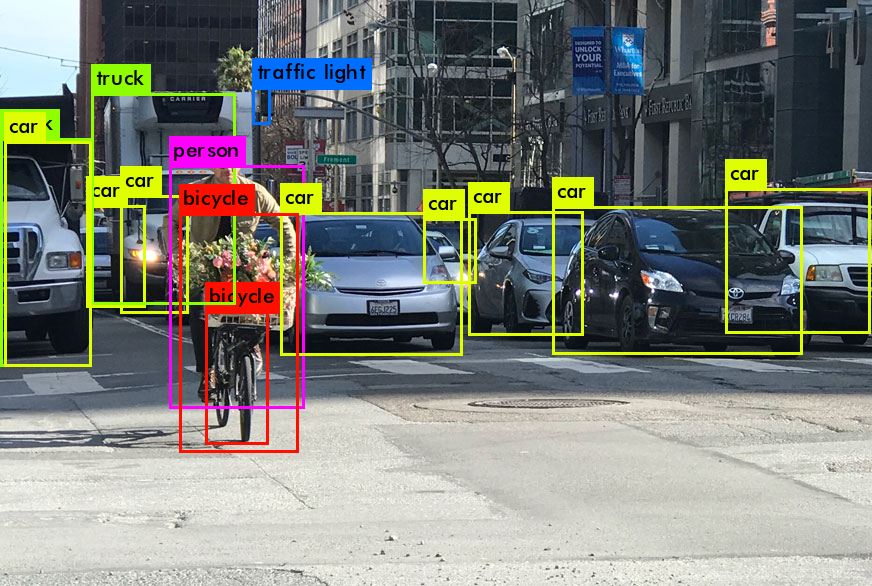
\includegraphics[width=\linewidth]{object_detection.png}
\caption{Predizione di un modello di Object Detection multiclasse}
\end{figure}

Da un'immagine fornita come input a un modello di Object Detection, verrà prodotto un file di testo, dove in ogni riga, sarà riportata una predizione di un'oggetto presente nell'immagine.
Per ciascuno degli oggetti individuati verrà riportato il numero identificativo della classe dell'oggetto (nel caso esista una sola classe il numero sarà sempre 0), la posizione dell'oggetto in formato xywh (posizione spaziale del centro e larghezza e altezza della box) oppure xyxy (coordinate rispettivamente dell'angolo superiore sinistro e inferiore destro della bounding box) e infine il valore di confidenza del modello per l'oggetto in questione. Questo ultimo parametro è particolarmente importante perchè permette a colui che utilizza o addestra la rete di ingorare predizioni al di sotto di un certo coeefficente di confidenza.\\ E' evidente come la scelta del coefficente di confidenza minimo sia molto delicata in quanto un valore alto riduce il numero di falsi positivi ma aumenta i falsi negativi e viceversa.\\
Formalizzando i concetti appena citati, nella prossima sezione definiremo i parametri fondamentali per la valutazione di un modello di Object Detection.
\subsection{Parametri di valutazione di un modello di Object Detection}
Le due metriche fondamentali per analizzare la perfomance di un modello sono la \emph{Precision} e la \emph{Recall}.
Rispettivamente, la \emph{Precision} fornisce un'indicazione sulla effettiva veredicità sulle predizioni fatte dal modello, la \emph{Recall} invece, ci da un'indicazione sul rapporto tra gli oggetti effetivamente individuati dalla rete e tutti quelli presenti nelle immagini.\\
Queste due importanti metriche, mostrano la loro correlazione nella curva \emph{Precision Recall curve}.
Formalizzando in formule abbiamo: 
\begin{align*}
Precision& = \frac{TP}{TP + FP}          &  Recall = \frac{TP}{TP + FN} \\
TP& = True \; positive    &  FN = True \; negative\\
FP& = False \; positive    &  FN = False \; negative
\end{align*}
Da questa curva, integrando è possibile ricavare un parametro molto informativo sulla qualità del modello, l'\emph{Average Precision, AP}.
\begin{equation}
    AP = \int_{0}^{1} p(r)dr
\end{equation}
Ovvero l'integrale sotto la curva Precision-Recall $p(r)$. Questo è il parametro principale per valutare la qualità di un modello nel riconoscimento di una specifica classe, poichè valuta conteporanemante sia la Precision che la Recall. \\
Se il modello ammette più classi, si calcola l'AP per ogni classe separatemnte e si fa la media del risultato, ottenendo la $mAP$.
\begin{equation}
    mAP = \frac{1}{n}\sum_{i=1}^{n}AP_{i}
\end{equation}
Dove $n$ è il numero di classi e $AP_{i}$ è l'integrale dalla curva Precision-Recall dell'$i$-esima classe.
Per avere un modello coerente bisuogna definire una metodologia per discriminare i True Positive dai False Positive in base alla posizione della bounding box disegnata dal modello rispetto a quella di label. \\
\begin{figure}[h]
\centering
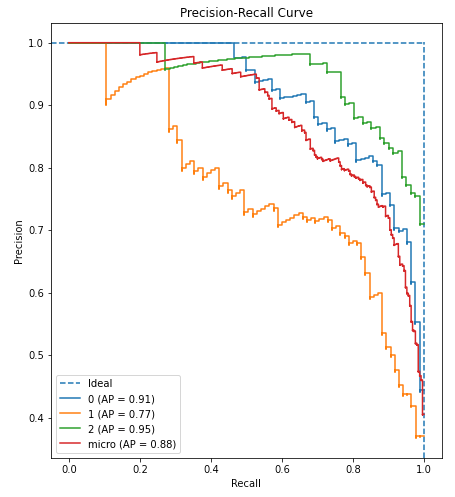
\includegraphics[width=300px,keepaspectratio]{precisionRecall2.png}
\caption{Curve Precision-Recall di vari modelli}
\end{figure}
\newpage
Per fare ciò si introduce il concetto di Interesection over Union (IoU). Ovvero, per ogni predizione del modello si calcola il rapporto tra l'intersezione delle due bounding boxes e la loro unione. \\
Quindi si scelgie un valore soglia arbitrario, a seconda delle esigenze del problema, al di sotto del quale la predizione del modello viene giudicata come non abbastanza precisa e quindi sbagliata. 
\\ Solo le predizioni del modello che soddifano il valore di soglia minimo della IoU vengono categorizzate come corrette e quindi concorrono positivamente al numero dei True Positive e quindi alla curva Precision.
\begin{figure}[h]
\centering
% 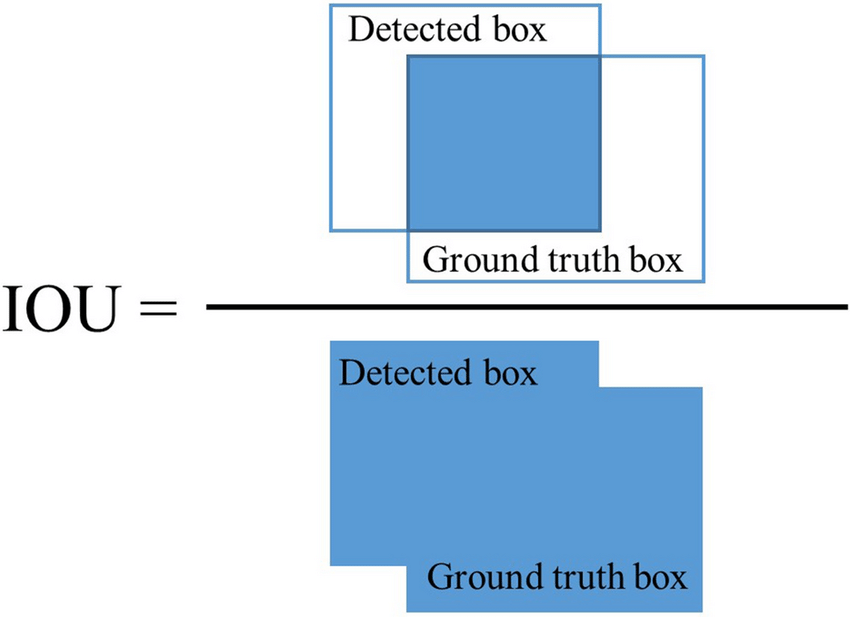
\includegraphics[width=\textwidth,height=\textheight,keepaspectratio]{IoU.png}
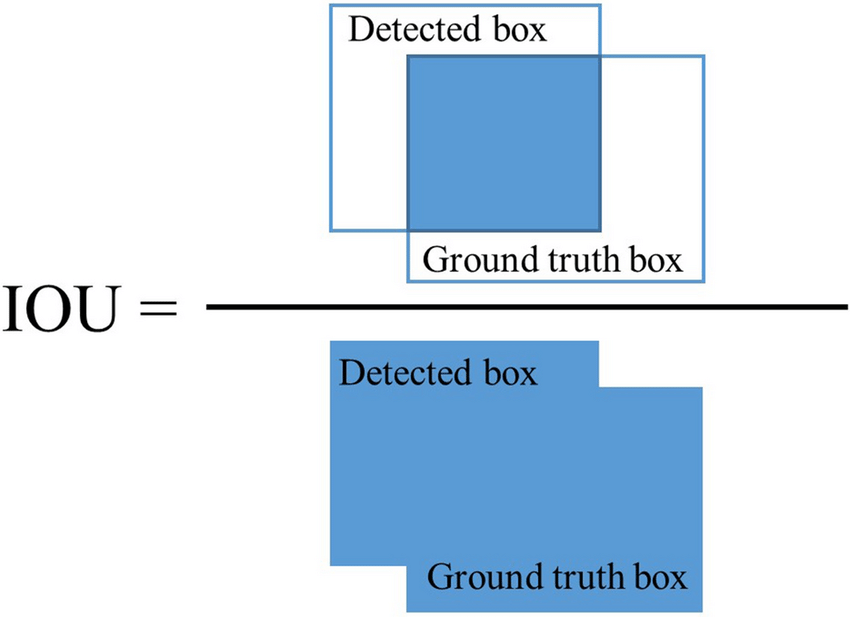
\includegraphics[width=\linewidth]{IoU.png}
\caption{Interesection over Union}
\end{figure}
Nella prossima sezione verrà analizzato il funzionamento e l'archiettura di YOLO, un noto modello allo stato dell'arte nella Object Detection, utilizzato nella sua ultima iterazione nel progetto su cui si basa questa tesi.
\newpage
\section{YOLO: You Look Only Once}
Il modello YOLO (You Look Only Once) è di fatto una delle soluzioni più popolari e utilizzate nelle applicazioni di Object Detection. In tutte le sue ierazioni ha avuto numerosissimi usi nei domini applicativi più diversi, come per esempio la guida autonoma grazie alla sua velocità di inferenza fondamentale nelle applicazioni real time. E' stato inotlre utilizzato nell'argricoltura, videosorveglianza, medicina, monitoraggio del traffico e molto altro.\\
In generale è stato sempre riconosciuto dalla comunità come uno strumento particolarmente equilibrato tra velocità di inferenza e precisione.\\
Con l'avanzare delle iterazioni sono state fatte modifiche di design della rete, modifiche alla funzione di costo, modifiche alle anchor box e molto altro. 
\\Nel caso applicativo del progetto svolto in questa tesi si è usato l'ultima iterazione YOLOv8, la più performante ma essendo essa ancora priva di paper, in questo elaborato ci si è dedicati all'analisi di YOLOv7.
\subsection{Funzionamento}
Come indicato dal nome, la rete propone un approccio a singolo stadio per il riconosicmento delle immagini. Molti dei modelli tradizionali di Object detection precedenti a YOLO utilizzano l'approccio a \emph{sliding window}, ovvero scannerizzano l'immagine facendo scorrere una finestra e a ogni nuova posizione utilizzavano un classificatore per controllare se all'interno della finestra fosse presente effettivamente un'oggetto. 
Questa tecnica, per quanto intuitiva è profondamente inefficente in qaunto per una sola immagina si utilizza un classificatore molte volte.
In generale comunque esistono una moltitudine di tecniche anche più avanzate che utilizzano comuque più stadi, dove per esempio il primo identifica le zone di interesse dell'immagine e successivamente un secondo stadio calssifica il contenuto all'interno. 
YOLO al contrario invece produce l'output con una sola regressione producendo in un solo passaggio sia le cordinate dell'oggetto che la propabilità della classe dell'oggetto trovato tutto nello stesso output.
Diferrente dall'approccio sliding window è per quello di \emph{Fast R-CNN}[R-CNN] che produce due output separati generati rispettivamente da un classificatore per la probabilità della classe e un regressore per la posizione della bounding box. In particolare R-CNN generara una serie di potenziali bounding boxes nell'immagine (region proposals), quindi inferisce un classificatore su ognuna di esse e infine utilizza una serie di tecniche a posteriori per eliminare bounding boxes doppie e ricalcolare le metriche delle singole predizioni in base alla posizione delle altre. Ognuno di questi metodi deve essere addestrato separatamente e una singola inferenza attarversa varie interezioni. 
\begin{figure}[h]
\centering

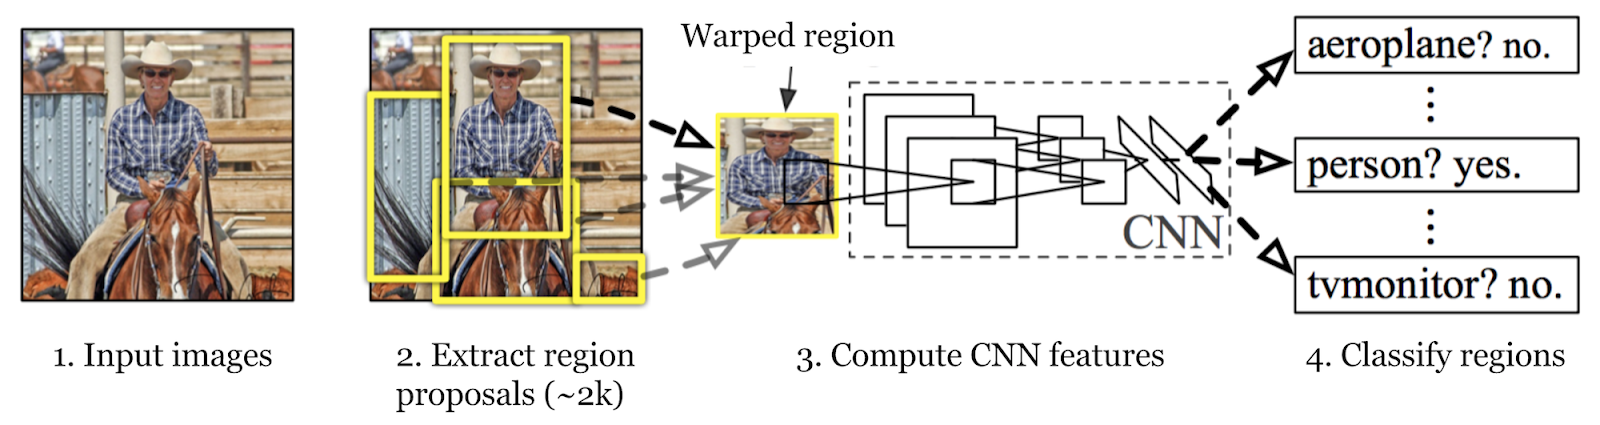
\includegraphics[width=\linewidth]{RCNN.png}
\caption{Funzionamento di R-CNN}
\end{figure}
Un'altro vantaggio di YOLO rispetto a R-CNN è quello di risucire a vedere tutta l'immagine durante il singolo step di inferenza, quindi considerando tutto il contesto e non solo i contesti delle singole region proposals. Questo porta a un notevole calo dei detect nelle zone di sfondo.

YOLO invece collassa tutto questo in un singolo problema di regressione. 
Per fare questo YOLO divide l'immagine di input in una griglia $S\times S$ e per ogni cella della griglia produce un numero $B$ di bounding boxes e i rispettivi punteggi di confidenza rispetto alle $C$ classi presenti nel problema per ognuna delle predizioni effettuate.
Nella fase finale effettiva solo le bounding boxes con confidenza al di sopra della soglia minima vengono effettivamente mostrate.

Per ogni boudning boxes YOLO produce 5 valori: $Pc,bx,by,bh,bw$, dove $Pc$ è detto \emph{confidence score} ovvero la confidenza del modello sulla possibiità che all'interno della regione sia effettivamente presente un oggetto, $bx$ e $by$ sono le coordinate del centro dell'oggetto relative alla cella della griglia. Infine $bh$ e $bw$ sono l'altezza e la larghezza della bounding box relativa all'intera immagine.
Per eliminare bounding box duplicate sovrapposte tra loro si utilizza la tecnica \emph{non-max supression} che rimuove le bounding box con il confidence score più basso quando la IoU delle due predizioni con la stessa classificazione è superiore a una solgia (solitamente 0.3). 

L'output di YOLO è quindi un tensore di grandezza $S \times S \times (B \times 5 + C)$
\begin{figure}[h]
\centering

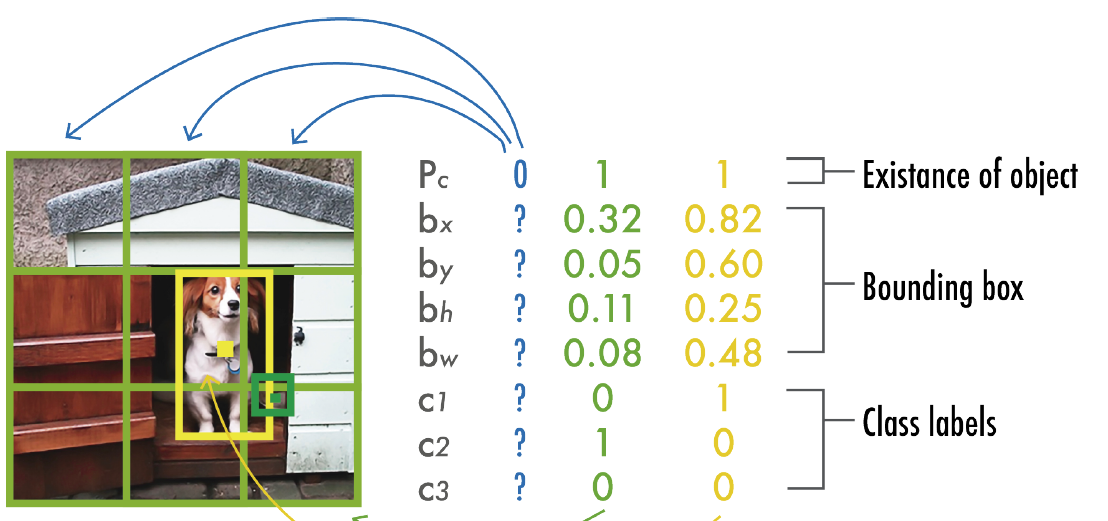
\includegraphics[width=\linewidth]{yoloOUTPUT.png}
\caption{Output di YOLO in un'immagine divisa con una griglia 3x3}
\end{figure}

\subsection{Architettura}
L'archiettettura del modello orginale YOLO è composta da 24 layer convoluzionali seguiti da due layer fully-connected che producono l'output delle coordinate delle bounding boxes e la classificazione degli oggetti. 
Tutti i layer utilizzano la funzione di attivazione chiamata \emph{leaky rectified linear unit}, la quale lascia invariati i valori positivi e divide per 10 quelli negativi. Mentre l'ultimo layer fully connected utilizza una funzione di attivazione lineare.
\begin{figure}[h]
\centering
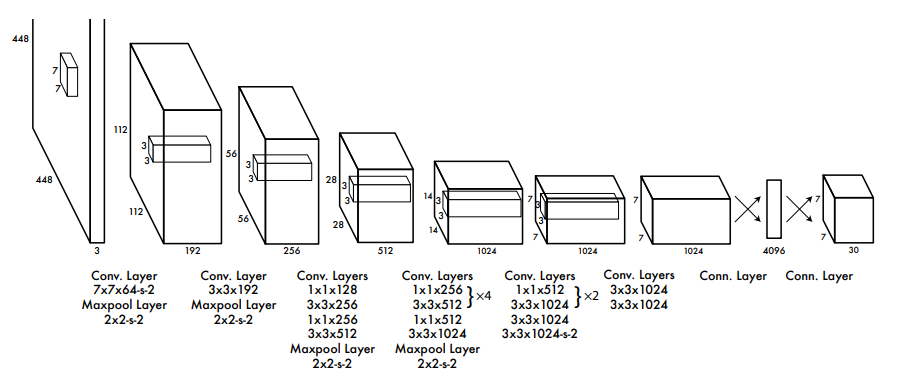
\includegraphics[width=\linewidth]{yolo1_arch.png}
\caption{Architettura YOLOv1}
\end{figure}
Con il tempo e il passare delle iterazioni YOLO ha ottenuto enormi sviluppi e modifiche architetturali. Qui ci limitiamo a citare le modifiche più importanti apportate con il passare delle versioni. 

A partire da YOLOv2 sono state introdotte le cosiddette \emph{anchor boxes}, ovvero delle bounding boxes di dimensioni predefinite preparate a priori per ogni cella della grglia. Queste boxes sono pensate per avere forme prototipate compatibili con le classi che si stanno cercando. L'output del modello, ovvero il numero di predizioni totali sarà pari al numero di anchor boxes per cella moltiplicato per il numero di celle.
\begin{figure}[h]
\centering
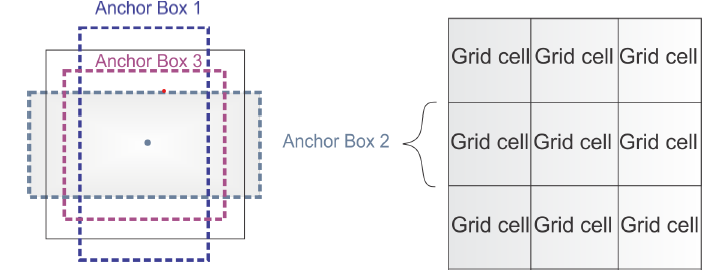
\includegraphics[width=\linewidth]{anchor.png}
\caption{Anchor boxes introdotte in YOLOv2}
\end{figure}
A partire da YOLOv3 inizia a delinearsi una struttura che marcherà la composizione di tutte le versioni successive, ovvero la scomposizione logica del modello in tre moduli separati con compiti diversi: Backbone, Neck, Head.
Il \emph{Backbone} è la prima parte del modello, quella di più basso livello. Questo modulo è tipicamente una rete puramente convoluzionale incaricata di estrapolare feature grafiche dall'immagine iniziale.
Il \emph{Neck} ha lo scopo di collegare la parte finale (Head) del modello con il Backbone. Questo modulo aggrega e affina le features passategli dal backbone enfatizzando tratti sementici e spaziali di più di alto livello rispetto a quelli estrapolati dal Backbone. 
Il modelo finale detto \emph{Head} si occupa di inferire le predizioni finali del modello sulla base delle features estratte dal Backbone e affinate dal Neck. E' composto da delle sottoreti incaricate di fare clasificazione e localizzazione degli oggetti. Inoltre sempre nella Head sono presenti moduli in grado di eliminare bounding boxes duplicate e altre operazioni post predizione.
\begin{figure}[h]
\centering
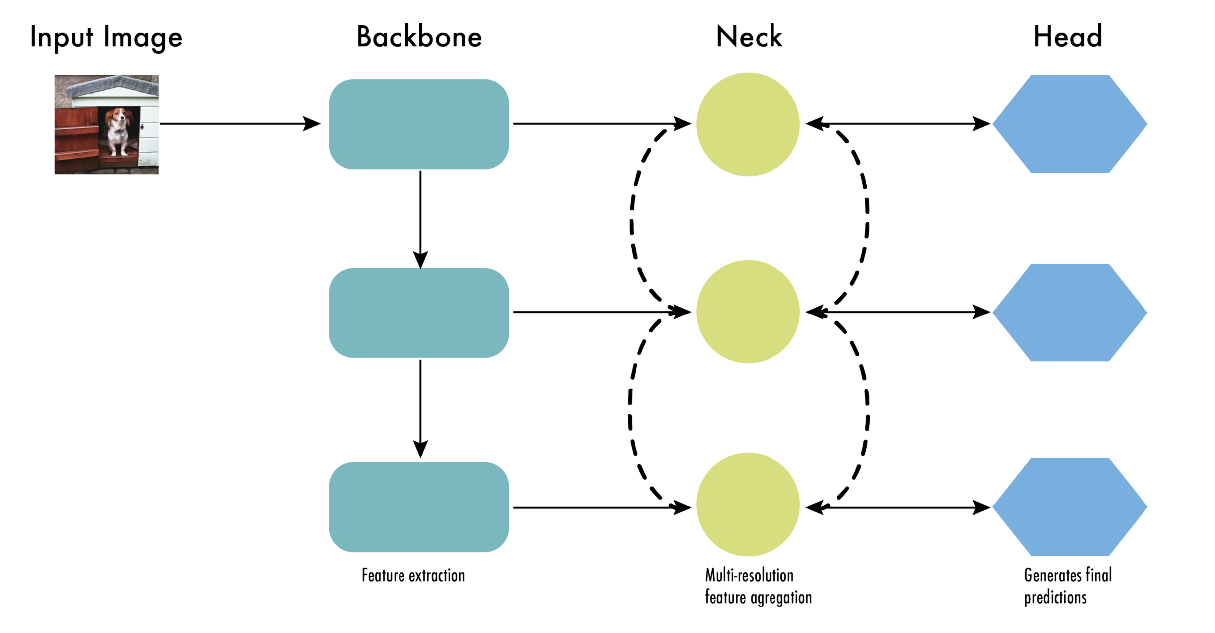
\includegraphics[width=\linewidth]{backbone_neck_head.png}
\caption{Archietettura con Backbone, Neck e Head}
\end{figure}
A partire da YOLOv4 le aggiunte al modello sono state divise in due distinte categorie, \emph{bag-of-freebies} e \emph{bag-of-specials}.
Le prime sono modifiche principalemente relative alle modalità di training, come per esempio la \emph{data augmentation}, ovvero la generazione di ulteriori immagini di imput facendo modifiche a quelle già utilizzate. Questa classe di modifiche ha un impatto negativo solo sul tempo di training e non su quello di inferenza. 
Un'interessante esempio di aggiunta di tipo \emph{bag-of-freebies} in YOLOv4 è stato l'inserimento di Algoritmi Genetici per l'ottimizzazione degli iperparametri di training.
Le aggiunte categorizzate come \emph{bag-of-specials} sono invece tipicamente modifiche strutturali che incidono sul tempo di inferenza migliorando però la precione finale.
\begin{figure}[h]
\centering
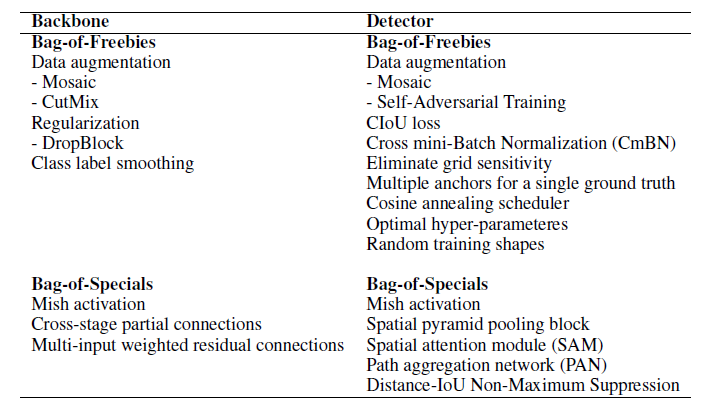
\includegraphics[width=\linewidth]{bagofreebies.png}
\caption{Lista di aggiunte e modifiche su YOLOv4 divise fra Bag-of-Freebies and Bag-of-Specials}
\end{figure}
Con YOLOv7 sono state introdotte modifiche architetturali piuttosto sofisticate come le \emph{Extended efficient layer aggregation network (E-ELAN)}, ovvero reti che si basano su metodi capaci di fare convergere più velocemente un generico modello di Deep Learning controllando la il percorso di discesa del gradiente ritenuto migliore dalla rete. 

Con YOLOv8 è stato fasso un grosso passo in avanti per quanto riguarda la facilità d'uso.
E' infatti possibile utilizzare il modello da un'interfaccia a riga di comando (CLI) oppure istallandolo nel propio ambiente di sviluppo Python come un pacchetto PIP. 
YOLOv8 viene rilascaito in 5 versioni differenti con diversi tradeoff tra performance e precisione.
Valutato sul dataset di riferimento COCO 2017 YOLOv8x ha raggiunto una AP di 53.9\% con immagini di 640 pixels rispetto al 50.7\% di YOLOv5 con una velocità di 280 immagini per secondo su una GPU NVIDIA A100. 

% \clearpage{\pagestyle{empty}\cleardoublepage}
% %%%%%%%%%%%%%%%%%%%%%%%%%%%%%%%%%%%%%%%%%per fare le conclusioni
% \chapter*{Conclusioni}
% %%%%%%%%%%%%%%%%%%%%%%%%%%%%%%%%%%%%%%%%%imposta l'intestazione di pagina
% \rhead[\fancyplain{}{\bfseries
% CONCLUSIONI}]{\fancyplain{}{\bfseries\thepage}}
% \lhead[\fancyplain{}{\bfseries\thepage}]{\fancyplain{}{\bfseries
% CONCLUSIONI}}
% %%%%%%%%%%%%%%%%%%%%%%%%%%%%%%%%%%%%%%%%%aggiunge la voce Conclusioni
%                                         %   nell'indice
% \addcontentsline{toc}{chapter}{Conclusioni} Queste sono le
% conclusioni.\\
% In queste conclusioni voglio fare un riferimento alla
% bibliografia: questo \`e il mio riferimento \cite{K3,K4}.
% %%%%%%%%%%%%%%%%%%%%%%%%%%%%%%%%%%%%%%%%%imposta l'intestazione di pagina
% \renewcommand{\chaptermark}[1]{\markright{\thechapter \ #1}{}}
% \lhead[\fancyplain{}{\bfseries\thepage}]{\fancyplain{}{\bfseries\rightmark}}
% \appendix                               %imposta le appendici
% \chapter{Prima Appendice}               %crea l'appendice
% In questa Appendice non si \`e utilizzato il comando:\\
% %%%%%%%%%%%%%%%%%%%%%%%%%%%%%%%%%%%%%%%%%\verb"" è equivalente all'
%                                         %   ambiente verbatim,
%                                         %   ma si utilizza all'interno
%                                         %   di un discorso.
% \verb"\clearpage{\pagestyle{empty}\cleardoublepage}", ed infatti
% l'ultima pagina 8 ha l'intestazione con il numero di pagina in
% alto.
% %%%%%%%%%%%%%%%%%%%%%%%%%%%%%%%%%%%%%%%%%imposta l'intestazione di pagina
% \rhead[\fancyplain{}{\bfseries \thechapter \:Prima Appendice}]
% {\fancyplain{}{\bfseries\thepage}}
% \chapter{Seconda Appendice}             %crea l'appendice
% %%%%%%%%%%%%%%%%%%%%%%%%%%%%%%%%%%%%%%%%%imposta l'intestazione di pagina
% \rhead[\fancyplain{}{\bfseries \thechapter \:Seconda Appendice}]
% {\fancyplain{}{\bfseries\thepage}}
\begin{thebibliography}{90}             %crea l'ambiente bibliografia
\rhead[\fancyplain{}{\bfseries \leftmark}]{\fancyplain{}{\bfseries
\thepage}}
%%%%%%%%%%%%%%%%%%%%%%%%%%%%%%%%%%%%%%%%%aggiunge la voce Bibliografia
                                        %   nell'indice
\addcontentsline{toc}{chapter}{Bibliografia}
%%%%%%%%%%%%%%%%%%%%%%%%%%%%%%%%%%%%%%%%%provare anche questo comando:
%%%%%%%%%%%\addcontentsline{toc}{chapter}{\numberline{}{Bibliografia}}
%-----------------------primo capitolo ------------------------
% textbook generale, molto completo sulle NN 
\bibitem{NN_book} R. Rojas, \emph{Neural Networks}, Springer-Verlag, Berlin, 1996
\bibitem{GD} Bottou, Léon; Bousquet, Olivier (2007). \emph{The Tradeoffs of Large Scale Learning}
%articolo sulla backpropagation
\bibitem{backprop} Annette Lopez Davila, Professor Chi-Kwong Li, \emph{Neural Networks: The Professor Chi-Kwong Li Algorithm} Math 400, College of William and Mary
%articolo sull'esempio del capitolo 1
\bibitem{handwritten} Ritik Dixit, Rishika Kushwah, Samay Pashine, \emph{Handwritten Digit Recognition using Machine and Deep Learning Algorithms}, Computer Science and Engineering
Acropolis Institute of Technology \& Research
Indore, India

%-----------------------secondo capitolo ------------------------
%CNN
\bibitem{cnn_overview}Rikiya Yamashita, Mizuho Nishio, Richard Kinh Gian Do Kaori Togashi \emph{Convolutional neural networks: an overview
and application in radiology}, Insights into Imaging volume 9, pages 611–629 (2018)
\bibitem{AP} Jesús María Romero Riveros, Prof. Piero Fraternali \emph{A metric evaluation framework for object detection}
\bibitem{yolo1}  Santosh Divvala, Ross Girshick, Ali Farhadi \emph{You Only Look Once: Unified, Real-Time Object Detection} University of Washington, Allen Institute for AI, Facebook AI Research

%articolo completo con storia, funzionamento e architettura di YOLO. Joseph Redmon∗
\bibitem{YOLO-story} Juan R. Terven, Diana M. Cordova-Esparaza, \emph{A comprehensive review of YOLO: From YOLOv1 to YOLOv8 and beyond}

\bibitem{YOLOv7_paper}Chien-Yao Wang, Alexey Bochkovskiy, Hong-Yuan Mark Liao \emph{YOLOv7: Trainable bag-of-freebies sets new state-of-the-art for real-time object
detectors}, Institute of Information Science, Academia Sinica, Taiwan
\end{thebibliography}
%%%%%%%%%%%%%%%%%%%%%%%%%%%%%%%%%%%%%%%%%non numera l'ultima pagina sinistra
% \clearpage{\pagestyle{empty}\cleardoublepage}
% \chapter*{Ringraziamenti}
% \thispagestyle{empty}
% Qui possiamo ringraziare il mondo intero!!!!!!!!!!\\
% Ovviamente solo se uno vuole, non \`e obbligatorio.
\end{document}
